%%% The main file. It contains definitions of basic parameters and includes all other parts.

%% Settings for single-side (simplex) printing
% Margins: left 40mm, right 25mm, top and bottom 25mm
% (but beware, LaTeX adds 1in implicitly)
\documentclass[12pt,a4paper]{report}
\setlength\textwidth{145mm}
\setlength\textheight{247mm}
\setlength\oddsidemargin{15mm}
\setlength\evensidemargin{15mm}
\setlength\topmargin{0mm}
\setlength\headsep{0mm}
\setlength\headheight{0mm}
% \openright makes the following text appear on a right-hand page
\let\openright=\clearpage

%% Settings for two-sided (duplex) printing
% \documentclass[12pt,a4paper,twoside,openright]{report}
% \setlength\textwidth{145mm}
% \setlength\textheight{247mm}
% \setlength\oddsidemargin{14.2mm}
% \setlength\evensidemargin{0mm}
% \setlength\topmargin{0mm}
% \setlength\headsep{0mm}
% \setlength\headheight{0mm}
% \let\openright=\cleardoublepage

%% Generate PDF/A-2u
\usepackage[a-2u]{pdfx}

%% Character encoding: usually latin2, cp1250 or utf8:
\usepackage[utf8]{inputenc}

%% Prefer Latin Modern fonts
\usepackage{lmodern}

%% Further useful packages (included in most LaTeX distributions)
\usepackage{amsmath}        % extensions for typesetting of math
\usepackage{amsfonts}       % math fonts
\usepackage{amsthm}         % theorems, definitions, etc.
\usepackage{bbding}         % various symbols (squares, asterisks, scissors, ...)
\usepackage{bm}             % boldface symbols (\bm)
\usepackage{graphicx}       % embedding of pictures
\usepackage{fancyvrb}       % improved verbatim environment
\usepackage[square,numbers]{natbib}         % citation style AUTHOR (YEAR), or AUTHOR [NUMBER]
\usepackage[nottoc]{tocbibind} % makes sure that bibliography and the lists
			    % of figures/tables are included in the table
			    % of contents
\usepackage{dcolumn}        % improved alignment of table columns
\usepackage{booktabs}       % improved horizontal lines in tables
\usepackage{paralist}       % improved enumerate and itemize
\usepackage{xcolor}         % typesetting in color
\usepackage{subcaption}    
\usepackage{afterpage}
\usepackage{makecell}
\usepackage{cleveref}
\usepackage{booktabs}
\usepackage{multirow}
\usepackage{enumitem}
\usepackage{listings}
\usepackage{algorithm}
\usepackage[noend]{algpseudocode}
\newcommand\mycommfont[1]{\footnotesize\ttfamily{#1}}
\usepackage{enumitem}
\newlist{steps}{enumerate}{1}
\setlist[steps, 1]{label = Step \arabic*}

%%% Basic information on the thesis

% Thesis title in English (exactly as in the formal assignment)
\def\ThesisTitle{Constrained Spectral Uplifting}

% Author of the thesis
\def\ThesisAuthor{Bc. Lucia Tódová}

% Year when the thesis is submitted
\def\YearSubmitted{2020}

% Name of the department or institute, where the work was officially assigned
% (according to the Organizational Structure of MFF UK in English,
% or a full name of a department outside MFF)
\def\Department{Department of Software and Computer Science Education}

% Is it a department (katedra), or an institute (ústav)?
\def\DeptType{Department}

% Thesis supervisor: name, surname and titles
\def\Supervisor{doc. Alexander Wilkie, Dr.}

% Supervisor's department (again according to Organizational structure of MFF)
\def\SupervisorsDepartment{Department of Software and Computer Science Education}

% Study programme and specialization
\def\StudyProgramme{Computer Science}
\def\StudyBranch{Computer Graphics and Game Development}

% An optional dedication: you can thank whomever you wish (your supervisor,
% consultant, a person who lent the software, etc.)
\def\Dedication{%
I would like to express my sincere gratitude to my supervisor doc. Alexander Wilkie, Dr., for his time, guidance and patience over the last year.
I would also like to thank my boyfriend, my family and my friends for their constant support.
}

% Abstract (recommended length around 80-200 words; this is not a copy of your thesis assignment!)
\def\Abstract{%
Abstract.
}

% 3 to 5 keywords (recommended), each enclosed in curly braces
\def\Keywords{%
{key} {words}
}

%% The hyperref package for clickable links in PDF and also for storing
%% metadata to PDF (including the table of contents).
%% Most settings are pre-set by the pdfx package.
\hypersetup{unicode}
\hypersetup{breaklinks=true}

% Definitions of macros (see description inside)
%%% This file contains definitions of various useful macros and environments %%%
%%% Please add more macros here instead of cluttering other files with them. %%%

%%% Minor tweaks of style

% These macros employ a little dirty trick to convince LaTeX to typeset
% chapter headings sanely, without lots of empty space above them.
% Feel free to ignore.
\makeatletter
\def\@makechapterhead#1{
  {\parindent \z@ \raggedright \normalfont
   \Huge\bfseries \thechapter. #1
   \par\nobreak
   \vskip 20\p@
}}
\def\@makeschapterhead#1{
  {\parindent \z@ \raggedright \normalfont
   \Huge\bfseries #1
   \par\nobreak
   \vskip 20\p@
}}
\makeatother

% This macro defines a chapter, which is not numbered, but is included
% in the table of contents.
\def\chapwithtoc#1{
\chapter*{#1}
\addcontentsline{toc}{chapter}{#1}
}

% Draw black "slugs" whenever a line overflows, so that we can spot it easily.
\overfullrule=1mm

%%% Macros for definitions, theorems, claims, examples, ... (requires amsthm package)

\theoremstyle{plain}
\newtheorem{thm}{Theorem}
\newtheorem{lemma}[thm]{Lemma}
\newtheorem{claim}[thm]{Claim}

\theoremstyle{plain}
\newtheorem{defn}{Definition}

\theoremstyle{remark}
\newtheorem*{cor}{Corollary}
\newtheorem*{rem}{Remark}
\newtheorem*{example}{Example}

%%% An environment for proofs

\newenvironment{myproof}{
  \par\medskip\noindent
  \textit{Proof}.
}{
\newline
\rightline{$\qedsymbol$}
}

%%% An environment for typesetting of program code and input/output
%%% of programs. (Requires the fancyvrb package -- fancy verbatim.)

\DefineVerbatimEnvironment{code}{Verbatim}{fontsize=\small, frame=single}

%%% The field of all real and natural numbers
\newcommand{\R}{\mathbb{R}}
\newcommand{\N}{\mathbb{N}}

%%% Useful operators for statistics and probability
\DeclareMathOperator{\pr}{\textsf{P}}
\DeclareMathOperator{\E}{\textsf{E}\,}
\DeclareMathOperator{\var}{\textrm{var}}
\DeclareMathOperator{\sd}{\textrm{sd}}

%%% Transposition of a vector/matrix
\newcommand{\T}[1]{#1^\top}

%%% Various math goodies
\newcommand{\goto}{\rightarrow}
\newcommand{\gotop}{\stackrel{P}{\longrightarrow}}
\newcommand{\maon}[1]{o(n^{#1})}
\newcommand{\abs}[1]{\left|{#1}\right|}
\newcommand{\dint}{\int_0^\tau\!\!\int_0^\tau}
\newcommand{\isqr}[1]{\frac{1}{\sqrt{#1}}}

%%% Various table goodies
\newcommand{\pulrad}[1]{\raisebox{1.5ex}[0pt]{#1}}
\newcommand{\mc}[1]{\multicolumn{1}{c}{#1}}


% Title page and various mandatory informational pages
\begin{document}
%%% Title page of the thesis and other mandatory pages

%%% Title page of the thesis

\pagestyle{empty}
\hypersetup{pageanchor=false}
\begin{center}

\centerline{\mbox{
\includegraphics[width=166mm]{img/logo-en.pdf}}}

\vspace{-8mm}
\vfill

{\bf\Large MASTER THESIS}

\vfill

{\LARGE\ThesisAuthor}

\vspace{15mm}

{\LARGE\bfseries\ThesisTitle}

\vfill

\Department

\vfill

{
\centerline{\vbox{\halign{\hbox to 0.45\hsize{\hfil #}&\hskip 0.5em\parbox[t]{0.45\hsize}{\raggedright #}\cr
Supervisor of the master thesis:&\Supervisor \cr
\noalign{\vspace{2mm}}
Study programme:&\StudyProgramme \cr
\noalign{\vspace{2mm}}
Study branch:&\StudyBranch \cr
}}}}

\vfill

% Zde doplňte rok
Prague \YearSubmitted

\end{center}

\newpage

%%% Here should be a bound sheet included -- a signed copy of the "master
%%% thesis assignment". This assignment is NOT a part of the electronic
%%% version of the thesis. DO NOT SCAN.

%%% A page with a solemn declaration to the master thesis

\openright
\hypersetup{pageanchor=true}
\pagestyle{plain}
\pagenumbering{roman}
\vglue 0pt plus 1fill

\noindent
I declare that I carried out this master thesis independently, and only with the cited
sources, literature and other professional sources. It has not been used to obtain another
or the same degree.

\medskip\noindent
I understand that my work relates to the rights and obligations under the Act No.~121/2000 Sb.,
the Copyright Act, as amended, in particular the fact that the Charles
University has the right to conclude a license agreement on the use of this
work as a school work pursuant to Section 60 subsection 1 of the Copyright~Act.

\vspace{10mm}

\hbox{\hbox to 0.5\hsize{%
In \hbox to 6em{\dotfill} date \hbox to 6em{\dotfill}
\hss}\hbox to 0.5\hsize{\dotfill\quad}}
\smallskip
\hbox{\hbox to 0.5\hsize{}\hbox to 0.5\hsize{\hfil Author's signature\hfil}}

\vspace{20mm}
\newpage

%%% Dedication

\openright

\noindent
\Dedication

\newpage

%%% Mandatory information page of the thesis

\openright

\vbox to 0.5\vsize{
\setlength\parindent{0mm}
\setlength\parskip{5mm}

Title:
\ThesisTitle

Author:
\ThesisAuthor

\DeptType:
\Department

Supervisor:
\Supervisor, \SupervisorsDepartment

Abstract:
\Abstract

Keywords:
\Keywords

\vss}

\newpage

\openright
\pagestyle{plain}
\pagenumbering{arabic}
\setcounter{page}{1}


%%% A page with automatically generated table of contents of the master thesis

\tableofcontents

%%% Each chapter is kept in a separate file
\chapter*{Introduction}
\addcontentsline{toc}{chapter}{Introduction}


\chapter{Color Science}

Color science, or colorimetry, is a branch of science that concerns itself with human perception of color. It researches the relations between human vision and physical properties of color, and analyzes options for both its capturing and reconstruction.

We begin this chapter by describing the physical properties of light and their subsequent meaning in terms of color. We then provide multiple options for quantifying said color for further possible reconstruction in the digital world. Lastly, we show the importance of color representation in modern-day renderers, and its effects of physically based phenomena.

\section{Light and Color}

Human visual perception refers the ability of the human eye to interpret the surrounding environment. It is based on our capability to detect \emph{electromagnetic radiation}, which is a form of energy that consists of waves which propagate through space and transmit radiant energy.

An \emph{electromagnetic wave} is characterized by its \emph{amplitude} and \emph{frequency}. Amplitude is defined as the distance between the central axis and either the \emph{crest} (the highest point of the wave) or the \emph{trough} (the lowest point of the wave), while frequency specifies how many wave cycles occur in a second. Together, these properties give rise to the term \emph{wavelength}, denoted $\lambda$, which measures the length of the wave --- the distance between either two subsequent crests, troughs or any two following spots with the same height. 

Every electromagnetic wave can be unambiguously defined by its wavelength. Arranging them according to this criterion creates a classification known as \emph{electromagnetic spectrum} (see~\cref{fig:electromagneticSpectrum}). As the electromagnetic spectrum contains all existing types of electromagnetic radiation, it covers wavelengths in the range from fractions of nanometers to thousands of kilometers. This range can be divided into bands to distinguish known types of electromagnetic waves, from low frequency gamma or X-rays to high frequency radio waves. 

\begin{figure}[t]
	\centering
	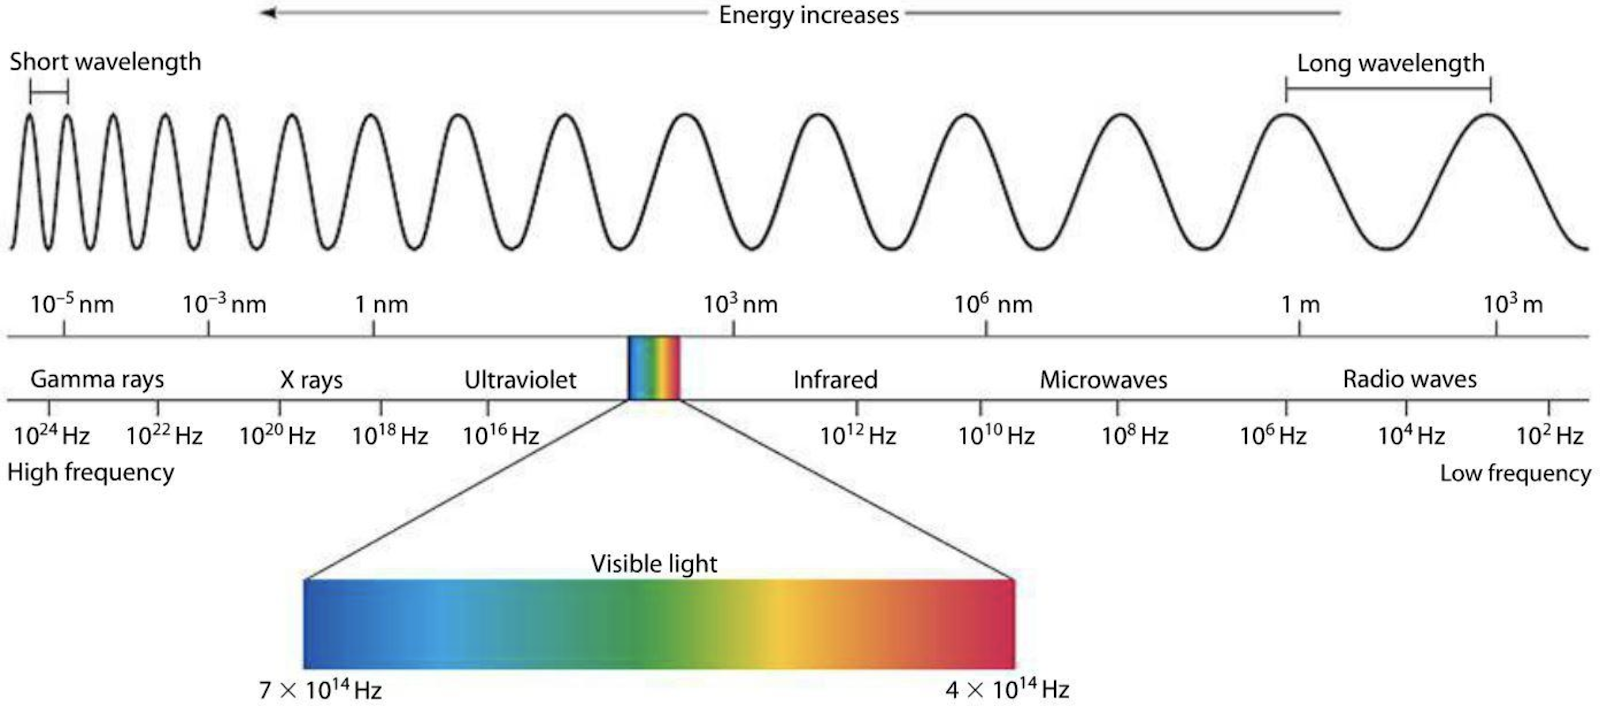
\includegraphics[width=0.8\linewidth]{img/electromagnetic_spectrum.png}
	\caption{An illustration of the electromagnetic spectrum~\cite{electromagneticSpectrum}} \label{fig:electromagneticSpectrum}
\end{figure}

In this thesis, we focus on \emph{visible light}, which covers only a mere fraction of the electromagnetic spectrum. Its waves are roughly in the 380-780nm range.

To sum up, electromagnetic waves specify the way in which light travels. To, however, describe the interaction between light and matter, the term \emph{photon} is used.

Photons are elementary particles of light moving in a manner specified by their wavelengths. They make up electromagnetic radiation and can be emitted or absorbed by atoms and molecules. During this process, they transfer energy either from the object that emitted them or to the object that absorbed them. This change in energy (denoted $E$) is proportional to the wave frequency of the absorbed/emitted photon and can be computed as follows~\citep{planckConstant}: 
\begin{equation} \label{energyEquation}
E = hf = \dfrac{hc}{\lambda}
\end{equation}
where $h$ is Planck's constant, $f$ is the frequency and $c$ is the speed of light. Therefore, generally speaking, the human eye identifies light when atoms and molecules in the retina absorb photons. 

To specify this process, we will first describe the retina. The retina consists of millions of light-sensitive cells, also called \emph{photoreceptors}, which pass a visual signal via an optic nerve to the brain, giving the notion of light and color. There are two types of photoreceptors in the human eye --- rods and cones.

\emph{Rods} make up most of the receptor cells (around 91 million according to~\citet{rods91cones4f5}, but other sources state that their number could be as high as 125 million~\cite{rods125cones6}). They are usually located around the boundary of the retina, and are responsible for low light (\emph{scotopic}) vision. However, they possess very little notion of color, which is also the reason why the human eye has trouble recognizing colors during the night.

\emph{Cones} are located mainly in the center of the retina and their numbers are a lot lower (from around 4.5 million~\cite{rods91cones4f5} to 6 million~\cite{rods125cones6}). In contrast to rods, they are active at daylight levels (responsible for \emph{photopic} vision) and have the notion of color. To be specific, different types of cones differ in their sensitivity to photon energies at concrete wavelengths. The final color is then composed by the brain from the stimulation signals sent by each cone.

The human eye has three types of cones:
\begin{itemize}
	\item \emph{L-cones}, which are the most responsive to longer wavelengths at around 560nm. When stimulated, they correspond to the red color
	\item \emph{M-cones}, which are the most sensitive to medium wavelengths at around 530nm and correspond to green color
	\item \emph{S-cones}, which respond the most to small wavelengths that peak at around 420nm and correspond to blue color
\end{itemize}

Their relative response to stimulation can be seen in~\cref{fig:coneSensitivity}.
\begin{figure}[t]
	\centering
	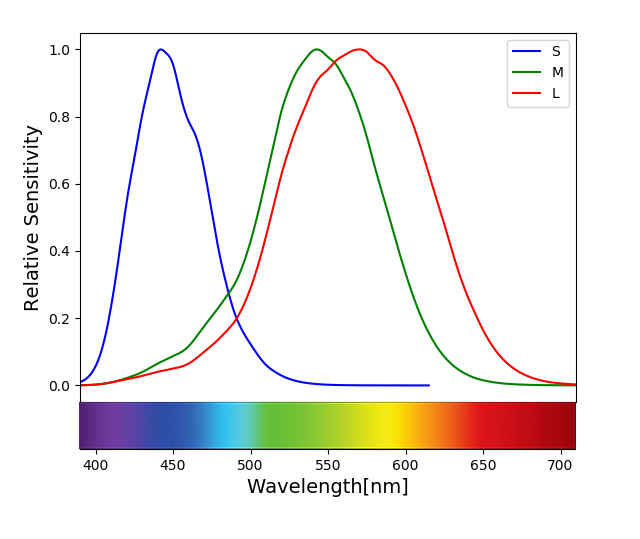
\includegraphics[width=0.5\linewidth]{img/cone_sensitivity.png}
	\caption{Relative sensitivity of S, M and L-cones plotted according to the data measured by~\citet{coneSensitivities}.} \label{fig:coneSensitivity}
\end{figure}

This type of color perception is called \emph{trichromatic}, as it uses three types of receptors to create the whole color space. The attempts to simulate such perception in the digital world give rise to tristimulus color representations, which have been widely adapted in color science. We discuss these thoroughly in~\cref{sec:colorRepresentation}.

Up until now, we have been talking about the interaction of light with the human eye. Photons, however, also interact with objects. As established by the relationship defined in~\cref{energyEquation}, the energy transferred to an object upon light interaction is dependent on the photon wavelength. This means that objects might absorb some wavelengths and reflect others.

Object color is defined by the wavelengths it \emph{reflects}. For example, if it reflects all the wavelengths, the resulting color is white, while absorbing all the wavelengths would render the object black. Naturally, human perception of object color is not only dependent on its reflective properties, but also on the lighting of the scene. If the only present light is red, wavelengths corresponding to colors other than red never hit the object. Therefore, the object might reflect only a subset of wavelengths than it would under white light, which may subsequently result in a change of the perceived color.

\section{Color representation} \label{sec:colorRepresentation}

The question of how to discretely represent color has been posed ever since the introduction of the first graphical user interface. For use in computer science, representations are required to be compact, precise, and the operations on colors to be easily executed.

We have already briefly mentioned the tristimulus representation in the previous section. In this section, we will overview its basic properties and describe some of the most popular tristimulus systems. We will also talk about an alternative representation, based primarily on the physical properties of color --- the spectral representation.

\subsection{Spectral representation}

When defining the color of an object, we must not only specify the wavelengths it reflects, but also the ratio between the incoming and the outgoing energy at these wavelengths. The dependency of reflectance on the wavelength is called a \emph{reflectance spectrum}, and is usually a smooth, continuous curve (see example in~\cref{fig:spectralRepres_reflectance}).

Although this definition might be sufficient for reflective surfaces, describing the color emitted by a light source requires the knowledge of the source's power rather than reflectance. For these purposes, \emph{spectral power distribution} (SPD) is used. Generally, SPD is a function describing the relationship between wavelength and any radiometric or photometric quantity (radiant energy, luminance, luminous flux, irradiance et cetera\ldots). In this thesis, however, we use SPD to describe the emissive properties of light sources, and therefore consider SPD to be a function of wavelength and power. We provide an example of an emission spectrum in~\cref{fig:spectralRepres_illuminant}.

\begin{figure}[t]
	\centering
	\begin{subfigure}[t]{0.31\textwidth}	
		\captionsetup{justification=centering}
		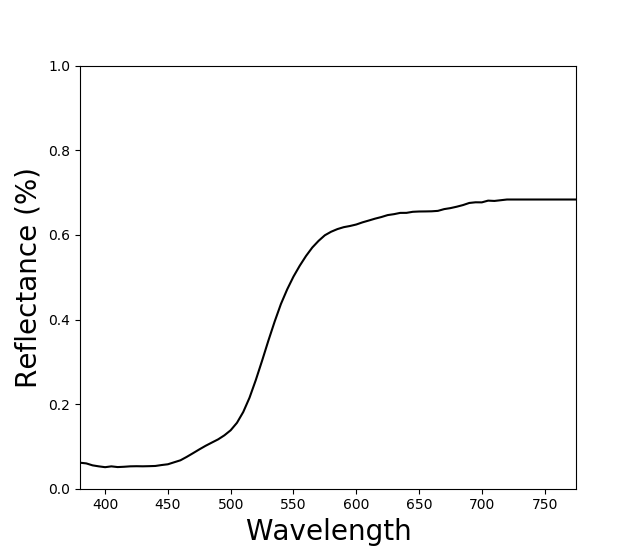
\includegraphics[width=\linewidth]{img/spectralRepres_reflectance.png}
		\caption{Reflectance spectrum (``orange yellow'' patch of Macbeth Color Chart)}
		\label{fig:spectralRepres_reflectance}
	\end{subfigure}
	\begin{subfigure}[t]{0.31\textwidth}
	\captionsetup{justification=centering}
	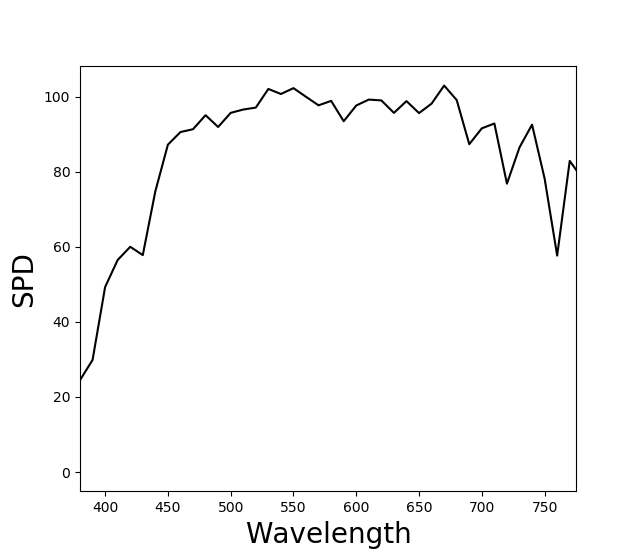
\includegraphics[width=\linewidth]{img/spectralRepres_emission.png}
	\caption{Emission spectrum (D50 illuminant) }
	\label{fig:spectralRepres_illuminant}
	\end{subfigure}
	\begin{subfigure}[t]{0.31\textwidth}
	\captionsetup{justification=centering}
	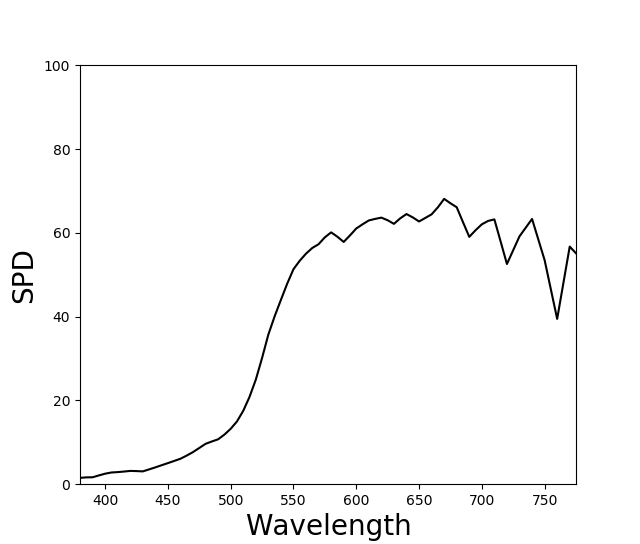
\includegraphics[width=\linewidth]{img/spectralRepres_combination.png}
	\caption{``orange yellow'' patch of Macbeth Color Chart illuminated by D50}
	\label{fig:spectralRepres_combination}
	\end{subfigure}
	\caption{The behavior of a reflectance of a surface under an illuminant}
	\label{fig:spectralRepresExamples}
\end{figure}

The color of an object illuminated by a light source can be determined by multiplying the light source's SPD curve with the reflectance curve of the object, as shown in an example in~\cref{fig:spectralRepresExamples}. This way the physical properties of color are preserved and the results are the same as they would be in nature.

\subsection{Tristimulus representation} \label{ssec:tristimulusRepres}

The obvious drawback of spectral representation is the difficulty of its discretization, since there is an infinite number of possible spectral curves, but only a finite number of digital colors that can be displayed by a monitor. For the purposes of color visualization, a distinct, by nature discrete, color
representation is required. 

Tristimulus representation approaches this issue by saving the color as a set of three values. Although the original idea was to simulate the trichromatic perception of human eye (i.e. save values that specify how much have the red, green and blue cones been stimulated), over time, multiple other tristimulus color spaces have been created. They differ mostly in the range of colors they are capable of representing and in their practical use. Following, we provide an overview of some of the most popular ones.

\subsubsection{RGB color space}
The RGB color space is an additive space employing three primaries --- red, green and blue. In other words, if three lights with red, green and blue chromacities are used to illuminate a single point, any color within the RGB color space can be created solely by changing the lights' intensities. 

An RGB value can therefore be thought of as a point in a 3-dimensional Euclidean space with each of the coordinate axes representing one of the primaries. As the lights' intensities must be bounded, this space is narrowed down to a cube starting at the base of the coordinate system. Usually, the range for each value is defined within 0 and 255, but a normalized (0,1) range is also used.

Various implementations of the RGB color space exist. They differ in the specifications of the RGB primaries, and therefore in their \emph{color gamut}, which is the subset of colors they are capable of representing. Some examples (named in ascending order with respect to their color gamut) include ISO RGB, sRGB, Adobe RGB, Adobe Wide Gamut RGB and ProPhoto RGB. An illustrative comparison of the sRGB and Adobe RGB gamut in the chromaticity diagram (described thoroughly in~\cref{sssect:xyYcolorSpace}) can be seen in~\cref{fig:chromaticityDiagram}.

RGB color spaces are commonly used in everyday world, e.g. in LCD and LED displays, digital cameras, scanners and even in computer graphics rendering. Their main downside has, however, been discovered when designing color matching functions~\cite{colorMatchingDerivation}.

A \emph{color matching function} is a function designed to simulate the response of a certain type of cone in the human eye. In 1931, CIE designed a set of three color matching functions that could be used for spectral to RGB conversion~\cite{colorMatchingDerivation}. Denoted $\overline{r}(\lambda)$, $\overline{g}(\lambda)$ and $\overline{b}(\lambda)$, they approximate the response of the L, M and S cones respectively. However, as seen in figure~\cref{fig:colorMatchingRGB}, the functions may also acquire negative values. At the time, this posed a problem due to calculation errors. Therefore, to eliminate these negative portions of functions, CIE designed a new, imaginary color space --- the XYZ color space.

\begin{figure}[t]
	\centering
	\begin{subfigure}{0.46\textwidth}
		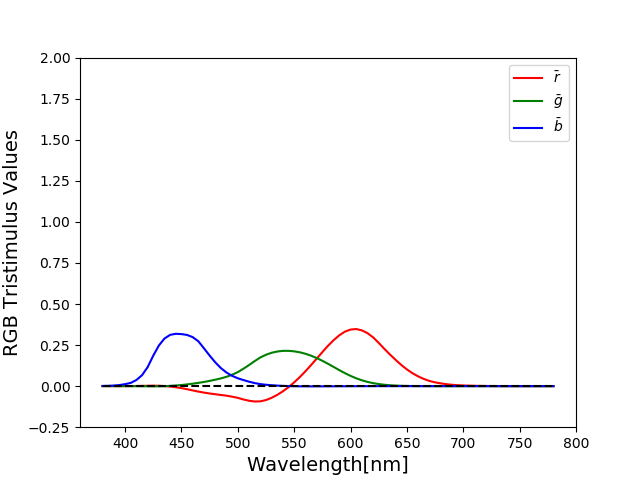
\includegraphics[width=\linewidth]{img/matching_functions_rgb.png}
		\caption{ $\overline{r}(\lambda)$, $\overline{g}(\lambda)$ and $\overline{b}(\lambda)$ functions plotted with data by~\citet{colorMatchingRGBData}}
		\label{fig:colorMatchingRGB}
	\end{subfigure}
	\quad
	\begin{subfigure}{0.46\textwidth}
		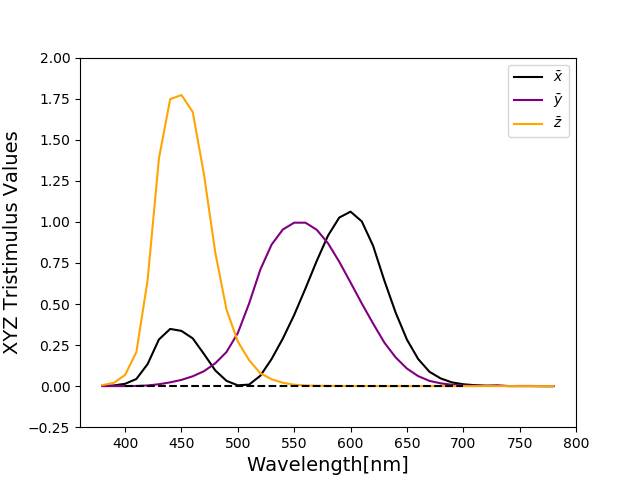
\includegraphics[width=\linewidth]{img/matching_functions_xyz.png}
		\caption{$\overline{x}(\lambda)$, $\overline{y}(\lambda)$ and $\overline{z}(\lambda)$ functions according to their spectral data from~\citet{colorMatchingXYZData}}
		\label{fig:colorMatchingXYZ}
	\end{subfigure}
	\caption{Color matching functions}
	\label{fig:colorMatchingFunctions}
\end{figure}

\subsubsection{XYZ color space}

The XYZ color space is a hypothetical color space capable of encompassing all colors perceptible by the human eye. Its color matching functions, $\overline{x}(\lambda)$, $\overline{y}(\lambda)$ and $\overline{z}(\lambda)$, were specifically designed for the purposes of SPD to tristimulus conversion, which is computed using the following equations:
\begin{equation} \label{spdToXYZ}
	\begin{aligned}
	X=\int P(\lambda)\overline{x}(\lambda)d\lambda,\\
	Y=\int P(\lambda)\overline{y}(\lambda)d\lambda,\\
	Z=\int P(\lambda)\overline{z}(\lambda)d\lambda,\\
	\end{aligned}
\end{equation}
where $X$, $Y$ and $Z$ are the resulting tristimulus values and $P(\lambda)$ is the spectral power distribution.

Although the X, Y and Z primaries were designed so that the Y primary closely matches luminance and X and Z primaries give color information, they are only imaginary, i.e. they do not correspond to any spectral distribution of wavelengths. This property renders the whole XYZ space imaginary, which means that it cannot be used for visualization purposes. Its main function is to serve as a ``middle step'' when performing a conversion from SPD to an arbitrary tristimulus space, which eliminates the need for creating color matching functions for other spaces. The conversion from XYZ into a tristimulus space can then be performed by a simple space-specific $3x3$ matrix transformation.

\subsubsection{xyY color space} \label{sssect:xyYcolorSpace}

In addition the impossible visualization process, another downside of the XYZ color space is that its values are practically unbounded and do not have any real meaning (such as the RGB triplets have). Therefore, a more intuitive color space has been created, which considers the relative proportions of the X, Y and Z values rather than their unbounded versions --- the xyY color space~\cite{xyYOverview}. It is based on the assumption that color can be regarded as a quantity with two properties: \emph{luminance} and \emph{chromaticity}.

The conversion from the XYZ to the xyY color space is performed as follows --- first, the $X$, $Y$ and $Z$ values are converted to their bounded versions (also called \emph{chromaticity coordinates}) as defined in~\cref{eq:XYZtoxyY}~\cite{xyYEquations}.
\begin{equation} \label{eq:XYZtoxyY}
\begin{aligned}
&x=\dfrac{X}{X+Y+Z}\\
&y=\dfrac{Y}{X+Y+Z}\\
&z=\dfrac{Z}{X+Y+Z}\\
\end{aligned}
\end{equation}
Since $x+y+z=1$, the $z$ term can be expressed as $z=1-x-y$. This means that $z$ does not give us any additional information about the current color and therefore can be dropped from the representation. It also implies that some information has been lost during the conversion, i.e. we cannot reconstruct the original XYZ triplet using only the $x$ and $y$ values and therefore cannot obtain the initial color. At least one of the original values is needed for this purpose ---~\citet{CIE} decided to use the $Y$ component, as it already specifies luminance.

Plotting the values of the $x$ and $y$ chromaticity coordinates creates a \emph{chromaticity diagram}, shown in~\cref{fig:chromaticityDiagram}. Each point of the curved boundary line (which is also called the \emph{spectral locus}) corresponds to a XYZ value that is the result of a monochromatic radiation (i.e. a single-wavelength stimulus). All other chromaticities visible to the standard observer lie within a region bounded by the spectral locus.

\begin{figure}[t!]
	\centering
	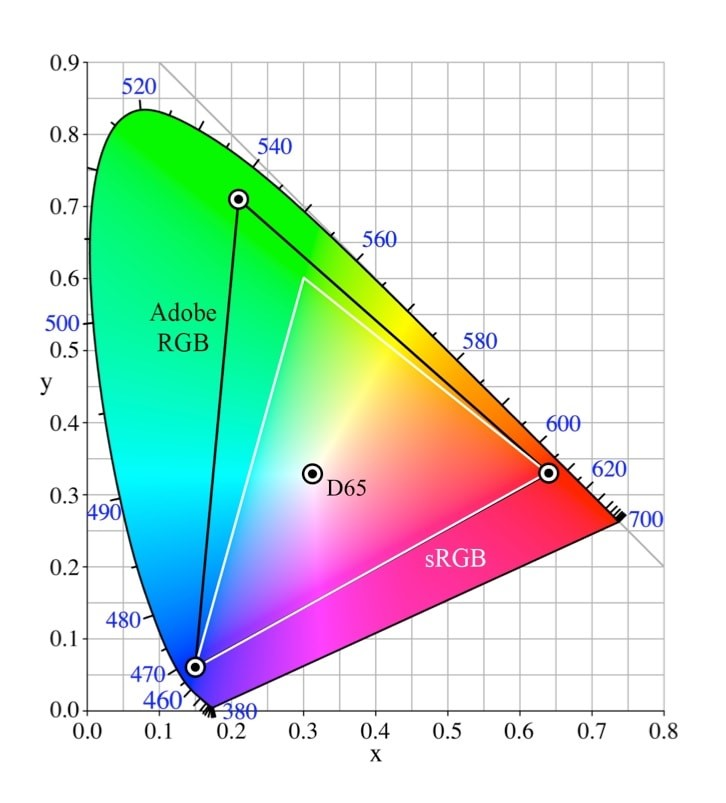
\includegraphics[width=0.6\linewidth,height=0.3\textheight]{img/chromaticity_diagram.jpeg}
	\caption{An illustrative comparison of the sRGB and Adobe RGB gamut in the chromaticity diagram based on images created by~\citet{chromaticityDiagramResource}}
	\label{fig:chromaticityDiagram}
\end{figure}

\subsubsection{L*a*b*}

Although some of the color spaces we have mentioned so far are already a lot more intuitive in terms of human color perception (e.g. xyY), neither of them regards for the human perception of color differences. The human eye is, for example, more prone to spotting differences when comparing lighter pastel colors and neglecting them upon interaction with darker color (e.g. dark blue). If we wish to accurately describe color differences in a color space, we must regard for this factor and aim for \emph{perceptual uniformity}, i.e. for the difference between two colors (as perceived by the human eye) to be proportional to their Euclidean distance within the color space.

The Hunter's Lab color space~\cite{hunterLabCIELabComparison} addressed this issue and was designed so that the distance between its two triplets characterized roughly how different they are in chromaticity and luminance. It is based on the Opponent color theory~\cite{opponentColorTheory}, which suggests that the cones in the human eye are linked together in opposing pairs and that the visual system records the \emph{difference} between the stimulation of the pairs rather than the cones' individual responses.

As the Hunter's Lab color space does not achieve perfect uniform spacing of values, CIE \emph{L*a*b*} color space (CIELAB) has been proposed in an attempt to improve some of its shortcomings and is now more widely used. However, neither of the systems are completely accurate in terms of perceptual uniformity~\cite{hunterLabCIELabComparison}.

The three opponent channels used to specify color in the CIE L*a*b* color space are defined as follows~\cite{labColorScale}:
\begin{itemize}
	\item \emph{L*} --- indicates lightness, i.e. the difference between \emph{light} and \emph{dark}. Its values range from $0$ (yielding black color) to $100$ (indicating diffuse white color)~\cite{labColorScale}.
	\item \emph{a*} --- defines the difference between \emph{green} and \emph{red}. Positives values of this component indicate the object's color to be more green, while negative values signify the domination of red.
	\item \emph{b*} --- defines the difference between \emph{yellow} and \emph{blue}. Positive values indicate the object to be more yellow, while negative values indicate the domination of blue.
\end{itemize}
Neither the range of the a* nor the b* component has any specific numerical limits~\cite{labColorScale}.

The L*a*b* color space is a \emph{reference system} --- an abstract, non-intuitive space encompassing all the human perceptible colors. Due to its perceptual uniformity, it can be used for color balance corrections by modifying the a* and b* components, and for lightness adjustments by modifying the L* component. However, as mentioned earlier, its main purpose is the determining of \emph{color differences}.

In 1976, CIE introduced the concept of \emph{Delta E}, which is the measure of change in visual perception of two colors~\cite{deltaEOverview}. Denoted $\Delta E_{ab}^*$, it is computed as an Euclidean distance between the two sample points, i.e.:
\begin{equation} \label{deltaE}
\Delta E_{ab}^*=\sqrt{(L_{2}^* - L_{1}^*)^2 + (a_{2}^* - a_{1}^*)^2 + (b_{2}^* - b_{1}^*)^2},
\end{equation}
where $(L_{1}^*,a_{1}^*,b_{1}^*)$ and $(L_{2}^*,a_{2}^*,b_{2}^*)$ are the L*a*b* coordinates of the sample points.

However, the $\Delta E_{ab}^*$ error is prone to exaggerate the differences occurring when comparing two highly saturated colors of similar hue. This is due to the fact that the L*a*b* color space is not perfectly perceptually uniform, which can be perceived upon observation of these regions. To improve upon these shortcomings, other measuring techniques for computing Delta E, such as Delta94 and Delta2000, have been proposed over the years.

\emph{Delta94} is computed by first modifying the original L*a*b* values of both colors to compensate for perceptual distortions in the color space and then by computing the Euclidean distance from the modified values. Although the results match the human color difference perception more closely, the Delta94 error metric still lacks some accuracy in the blue-violet region~\cite{deltaEOverview}.
	
\emph{Delta2000} attempts to remove these inaccuracies. Including the corrections added to Delta94, Delta2000 overall adds five correctional factors to the original $\Delta E_{ab}^*$ --- compensation factors for lightness, hue and chroma, compensation for neutral colors and, lastly, a hue rotation term for the problematic blue-violet region.

From the listed Delta E equations, the Delta2000 error measurements are the most accurate in terms of human color difference perception~\cite{deltaEOverview}. However, in addition to a complicated formula, the  DOPISAT. Therefore, we opt for using the simple $\Delta E_{ab}^*$ in the practical part of this thesis.

\subsubsection{Other color spaces}

In addition to the already mentioned tristimulus color spaces, there exist many more used for various purposes. Following, we briefly overview some of them:
\begin{itemize}
\item \emph{L*u*v*} --- Similarly to the CIELAB system, L*u*v* (or CIELUV) aims for perceptual uniformity. As a matter of fact, the $L*$ value is defined in the same manner as in the CIELAB system, while $u$ and $v$ values are evaluated by certain projections of the $x$ and $y$ coordinates of the chromaticity diagram. When comparing their Euclidean error measure, the most important distinction between the two spaces is that while the CIELAB generally improves CIELUV in terms of color difference~\cite{CIELABcomparisonCIELUV}, CIELUV does not have as many inaccuracies in the dark regions~\cite{CIELABDarkSide}. Therefore, it is often recommended to use the CIELUV color space for characterization of color displays and the CIELAB color space for the characterization of colored surfaces and dyes.

\item \emph{HSL} and \emph{HSI} color spaces define color by its \emph{hue}, \emph{saturation} and \emph{lightness} (or \emph{intensity}). They are an alternative representation of the RGB color space and must therefore be defined purely with reference to an RGB space~\cite{HSLreview}. As their components correlate better with human perception of color than those of the RGB system, they are often used in image processing applications, e.g. for processes such as feature detection (edge detection~\cite{edgeDetectionHSL}, object recognition) or image segmentation (which can be performed solely by using the hue component)~\cite{HSLreview}.

\item \emph{CMYK} model is a subtractive color model commonly used in color printing. It is based on RGB's complementary colors --- \emph{cyan}, \emph{magenta} and \emph{yellow} (respectively). This means that assigning zero values to all components renders white light, and increasing the value of a component specifies how much of the respective color is \emph{subtracted} from the white light. Although the premise is that maximizing CMY values should render perfect black, in reality, the printing inks are not 100\% pure CMY and their combinations therefore cannot produce rich black. For this purpose, a fourth component, \emph{black} ($K$), is often added, giving rise to the CMYK model.
\end{itemize}

Other color spaces include the Munsell color system, RAL, Natural Color System, Pantone Matching System, CIELCH\textsubscript{ab}, CIELCH\textsubscript{uv}, etc$\ldots$

\subsection{Color representation in rendering}

Accurate color representation is the core of rendering softwares. Although most of today's renderers support multiple color spaces, we can still divide them into two main categories according to the space used during evaluation of light transfer equations --- \emph{tristimulus} and \emph{spectral} renderers.

Tristimulus renderers are usually based on the RGB color space, although they often offer conversions to other tristimulus spaces. Due to the ease of use and simplicity of representation, RGB renderers are more common in commercial rendering software. They provide realistically looking images, often indistinguishable from a photograph, and are more robust, memory efficient and easy to implement.

\begin{figure}[t]
	\centering
	{\sffamily
		\begin{tabular}{cc}
			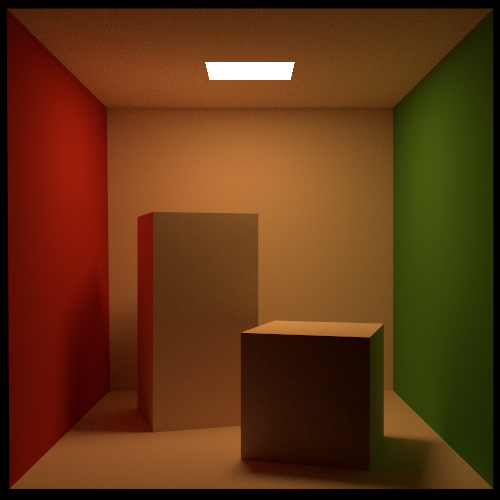
\includegraphics[width=0.45\linewidth]{img/mitsuba_rgb_mode.jpg}
			&
			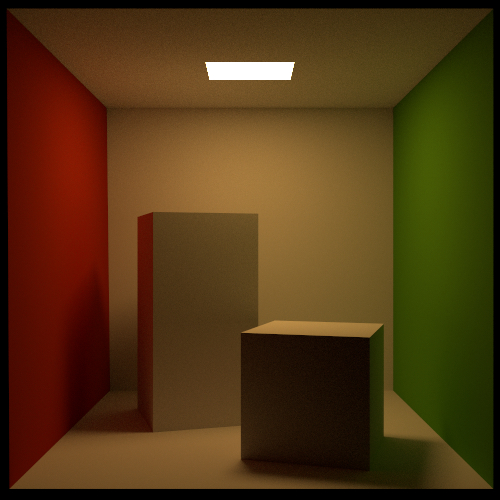
\includegraphics[width=0.45\linewidth]{img/mitsuba_spectral_mode.jpg}\\
		\end{tabular}
	}
	\caption{Comparison of an RGB-based rendering and spectral-based rendering as presented in the documentation of Mitsuba2~\cite{Mitsuba2}. Left: Spectral reflectance data of all materials is first converted to RGB and the scene is then rendered in the RGB mode, producing an unnaturally saturated image. Right: Scene is rendered directly in the spectral mode, resulting in more realistic colors. }
	\label{fig:mitsubaRGBSpectralComparison}
\end{figure}

However, light in real world does not travel as a tristimulus value, but rather as a distribution of wavelengths. Therefore, RGB renderers cannot properly simulate the physical properties of color during e.g. reflections or refractions when ray tracing.

Spectral rendering, on the other hand, uses full-spectral information of all materials and lights in the scene throughout the whole rendering process. Obviously, before visualization occurs, spectral information must be converted into tristimulus (usually RGB) values, but this does not pose a problem as, at the moment of conversion, all the physically based simulations have already taken place. Therefore, the rendered scene appears more realistic. We demonstrate this difference in~\cref{fig:mitsubaRGBSpectralComparison}, on a scene already rendered by Mitsuba2~\cite{Mitsuba2}.

In addition to a more convincing rendering of reflections and refractions, another reason for using spectral rendering is its capability to simulate physically based phenomena that arise due to the interaction of color with light. Following, we overview some of the most common ones:
\begin{itemize}
\item \emph{Metamerism} \label{item:metamerism}

As already mentioned in~\cref{ssec:tristimulusRepres}, the human tristimulus perception has a significantly lower domain than the (practically infinite) spectral domain. Therefore, two different spectra can trigger the same cone response in the human eye and appear to have the same color (and, subsequently, to have the same RGB values), giving rise to a phenomenon called \emph{metamerism}. The two spectra evaluating to the same tristimulus values are called \emph{metamers}.

In real world, metamerism is often perceived when the lighting conditions under which we observe metamers change. An example of this can be seen in~\cref{fig:metamerism}, where the color of the presented spheres is similar under the D65 illuminant, but clearly differs under the fluorescent F11 illuminant.

As an RGB renderer does not possess spectral information, it cannot replicate the behavior of spectral reflectance under an illuminant, and is therefore unable to reproduce metamerism.

\begin{figure}[t]
	\centering
	{\sffamily
		\begin{tabular}{cccc}
			Sphere reflectance curve & D65 Illuminant & F11 Illuminant 
			\vspace{1em} \\
			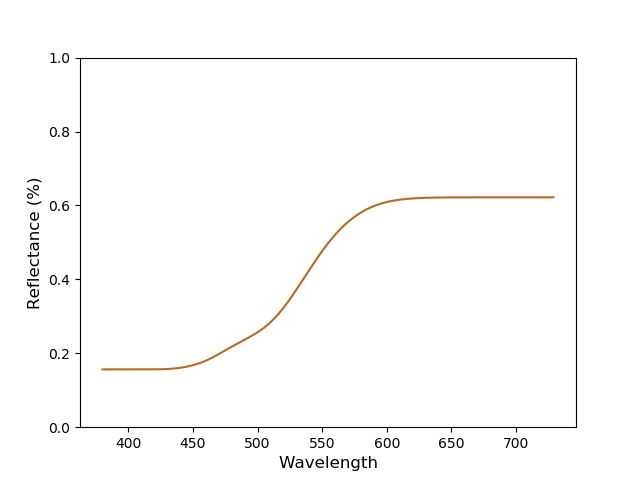
\includegraphics[width=.30\linewidth]{img/metamerism_first_curve.png}
			&
			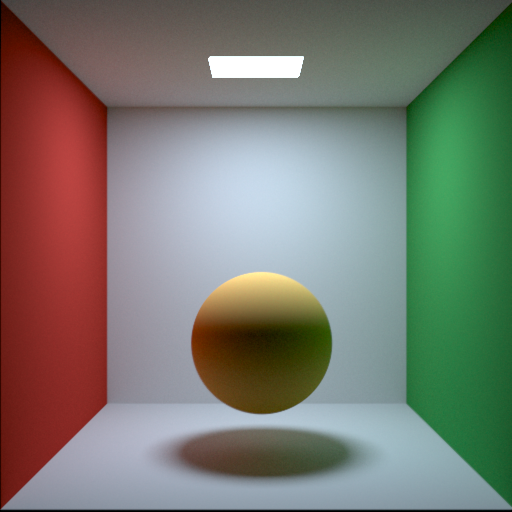
\includegraphics[width=.30\linewidth]{img/metamerism_first_d65.png}
			& 
			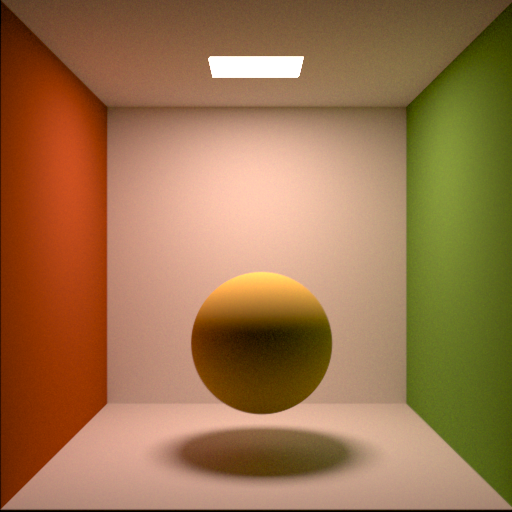
\includegraphics[width=.30\linewidth]{img/metamerism_first_fl11.png}
			\vspace{1em} \\
			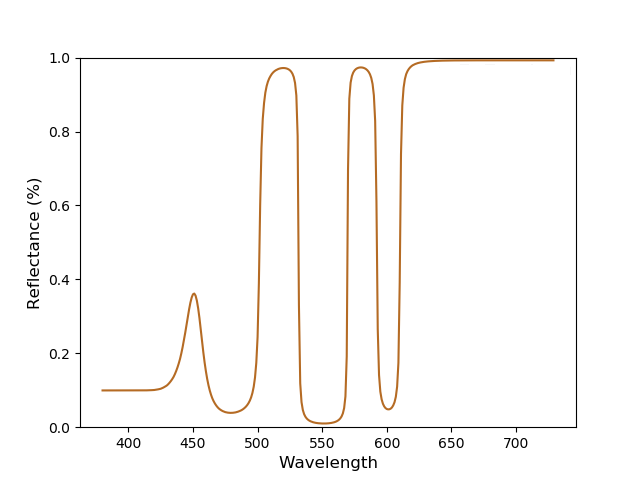
\includegraphics[width=.30\linewidth]{img/metamerism_second_curve.png}
			&
			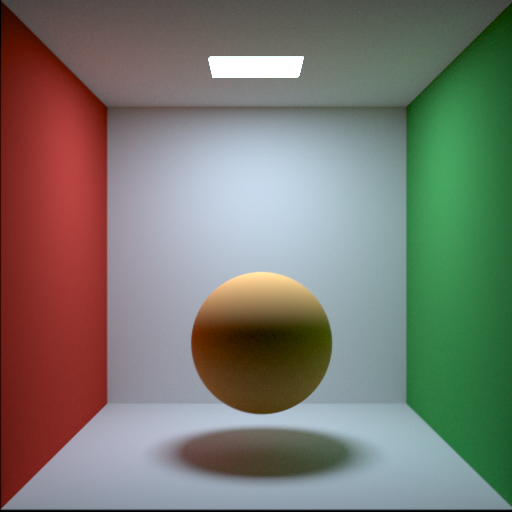
\includegraphics[width=.30\linewidth]{img/metamerism_second_d65.png}
			&
			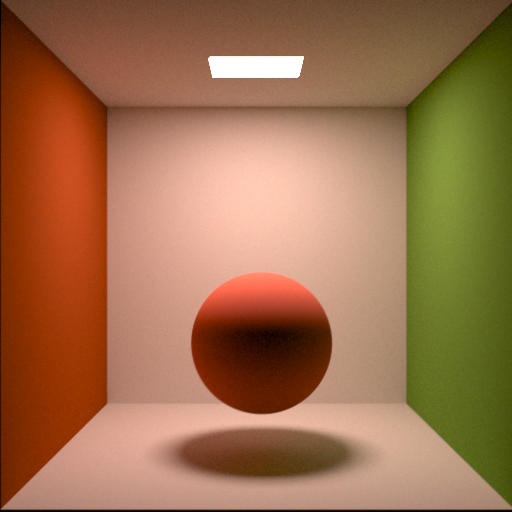
\includegraphics[width=.30\linewidth]{img/metamerism_second_fl11.png}
		\end{tabular}
	}
	\caption{The effects of metamerism. Left: Two different spectral reflectance curves, both evaluating to roughly $RGB=(220,175,105)$ under D65. Middle and right: Renderings of a sphere with assigned reflectance curves under D65 and F11 illuminants respectively.}
	\label{fig:metamerism}
\end{figure}

\item \emph{Fluorescence}

By definition, fluorescence occurs when light from one excitation wavelength $\lambda_0$ is absorbed by an object and is almost immediately re-emitted at a different, usually longer, wavelength $\lambda_1$~\cite{fluorescenceDefinition}. Specifically interesting is the fact that the absorbed light can come from outside of the visible spectrum and be re-emitted inside it, which results in an unrealistically bright appearance of materials. This can be perceived in real world when, for example, fish, corals, jellyfish or even minerals are illuminated by a UV light.

RGB renderers attempt to fake this kind of behavior through custom shaders~\cite{fluorescencePolarization}. As they often produce satisfactory results and, in comparison to physical simulation, are immensely easier to implement, physically based fluorescence has received small amount of work. Its support can be found in spectral renderers, added for example to ART by~\citet{fluorescenceART}.

\item \emph{Iridescence}

\emph{Iridescence}, or goniochromism, is a phenomenon occurring when certain surfaces change color according to the current viewing angle. It arises when the object's physical structure causes interferences between light waves (e.g. inside extremely thin dielectric layers), yielding rich color variations~\cite{iridescenceArticle1}. It can be perceived in nature in certain plants, specific minerals, butterfly wings, peacock's feathers, snakes, but also in man-made products such as oil leaks, soap bubbles or car paints.

Similarly to fluorescence, iridescent behavior can be ``faked'' in an RGB renderer~\cite{iridescenceRGB}. However, research based on physical properties of iridescence has also been conducted. For further information about the current development, we refer the interested reader to the articles by~\citet{iridescenceArticle1},~\citet{iridescenceArticle2}, or~\citet{iridescenceArticle3}.

\item \emph{Dispersion}

When light travels from one medium to another (e.g. when light coming from air hits glass or water), its direction of travel is changed. This phenomenon is called \emph{refraction} and is closely described by Snell's law, which specifies how the angle of refraction can be computed from the angle of incidence and the \emph{refraction indices} of the two media~\cite{snellsLaw}. However, the refraction index depends not only on the \emph{type} of media, but also on the current \emph{wavelength}~\cite{dispersionRendering1} --- which implies that the resulting direction of photons may vary according to their wavelength.

Probably the most known scenario displaying this phenomenon is white light hitting a dispersive prism. Upon interaction, light is split into a spectrum, creating a ``rainbow'' effect.

There have been multiple attempts to simulate physically based dispersion. We refer the interested reader to articles by~\citet{dispersionRendering1} or~\citet{dispersionRendering2}.

\item \emph{Polarization}

Electromagnetic waves traveling through space are \emph{transverse waves} --- their oscillation is perpendicular to their path of propagation. By default, the directions of oscillations are arbitrary for each photon --- this type of light is called an \emph{unpolarized light}. Restrictions to the directions of oscillations (also called \emph{polarization}) render \emph{polarized light}. Such phenomenon usually occurs upon light's interaction with certain materials.

The polarization process contributes to the overall color only in special cases (e.g. when using polarization filters)~\cite{fluorescencePolarization}. Therefore, it receives little attention in implementation of rendering softwares. However, for physical consistencies (and due to the possibility of unusual scenes) both ART~\cite{ART} and Mitsuba~\cite{Mitsuba2} follow the direction of oscillation during the rendering process.
\end{itemize}

Other researched phenomena (some of it closely linked to the already mentioned ones) include \emph{phosphorescence}, \emph{bioluminescence}, \emph{dichroism}, \emph{opalescence}, \emph{aventurescence} and many more.


\chapter{Spectral Uplifting}

Although spectral rendering has multiple advantages, many renderers do not consider them to compensate for the ease of use and memory efficiency of the RGB representation. Even the physically-based phenomena can be ``faked'' by a few simple tricks, and, therefore, many conventional rendering systems are RGB-based. This implies that most textures and materials created for renderers are also RGB-based.

However, spectral renderers are still used both in the research and in the commercial sphere (e.g. ART, Mitsuba, Manuka). In comparison to an RGB-based texture, however, creating spectral textures is much more complicated and usually requires a real-life model whose reflectance spectra can be measured with a spectrometer, which is, in many cases, virtually impossible. 

The obvious solution is to convert the already existing RGB models to their spectral variants. We refer to this process as \emph{spectral uplifting}, however, other sources also use the term \emph{spectral upsampling}~\cite{sigmoidMethod}. 

By being able to uplift RGB values, we could utilize the RGB textures and materials and therefore eliminate the need for a repeated creation of the textures from scratch by the tedious process of measuring specific spectral values.

However, converting an RGB value into its respective spectrum poses multiple difficulties. As the relationship between the spectral and RGB domain is not bijective (specifically, infinitely many spectral distributions render the same RGB values), distinctive approaches to the conversion process may render different spectral distributions. Although all of them might be correct in terms of the resulting RGB value, it is possible that none of them would be identical to spectral distribution measured with a spectrometer.

This does not cause a problem under standard illuminant with regard to which the RGB values were uplifted. However, as already mentioned in~\cref{item:metamerism}, changing the illuminant causes distinct spectra to behave differently, which consequently results in \emph{metamerism}. Therefore, our uplifted spectra might behave differently than they would in real world. sem dam obrazok ak ho budem mat

We begin this chapter by reviewing the already existing approaches to spectral uplifting. We then talk about a new technique, \emph{constrained spectral uplifting}, which provides means for solving the above mentioned problems.

\section{Uplifting methods} \label{sec:upliftingMethods}

Although there have been multiple attempts at spectral uplifting, not many meet all the conditions required for a successful and complete conversion (e.g. one method may output reflectance spectra with values outside the (0,1) range, other method might work only for saturated colors etc.).

We base most of this section on an article by~\citet{upsamplingTechniques}, as it overviews multiple spectral uplifting techniques. It also proposes a new technique, which is considered to be the current state-of-the-art.

One of the first techniques was proposed by~\citet{upsamplingMacAdam}. The main goal of his research was to achieve the highest possible brightness for a given color saturation in printing. The uplifting process was only a byproduct of proof of limits to the brightness of colors, created especially for representing the reflectance of the researched colors (i.e colors of maximum brightness for any given saturation). Although this method is not limited to a specific input, it produces spectra that are box shaped and only consist of rising and falling edges. This type of representation is unsuitable for colors usually found in nature, as they tend to have smooth spectra.

Another technique was proposed by~\citet{upsamplingSmits}. In this case, the uplifting is based on a box basis split into 10 discrete bins, which are derived using an optimization algorithm that accounts for energy conservation and aims for overall smoothness of the spectra. This approach is practically implemented and widely used, as it provides satisfactory results in the sRGB gamut~\cite{upsamplingJakobHanika}. However, in some cases, the uplifted spectra acquire values above 1, which does not satisfy the (0,1) range criterion. Furthermore, conversion of an RGB value to spectra and then back produces slight differences, which are amplified in scenes with multiple reflections. Lastly, this approach becomes unstable when used with wider gamuts, as it was not designed for this purpose.

The goal of the method by~\citet{upsamplingMeng} is wide-gamut uplifting. It also concentrates on optimizing the uplifting algorithm for spectral smoothness. However, it does not take energy conservation into account, which results in images with colors that have no physical counterpart (i.e. no real material could produce such colors). \citet{upsamplingMeng} try to solve this by introducing a set of scaling methods for mapping the uplifted spectra to valid reflectances. These, however, fail if trying to uplift bright colors. 

One of the most recent uplifting techniques has been proposed by~\citet{upsamplingOtsu}. It is based on the observation that a typical measured reflectance spectrum can be represented with only a few principle components. The method uses clustered principal component analysis (PCA) and, unlike many other approaches, does not assume that spectra must necessarily be smooth. Such a simplification both eliminates the requirement of having a smoothness heuristic and enables the reconstructed spectra to match the actual measured spectra pretty well. This approach, however, has its downsides. Firstly, the method does not satisfy the (0,1) range criterion. Therefore, the values must be clamped, which results in color reproduction errors. Moreover, since there is no interpolation across clusters, similar RGB values might produce very different spectra, which might lead to discontinuities in rendering. However, in multiple cases, this method has been shown to outperform all of the already mentioned ones~\cite{upsamplingJakobHanika}.

A large part of this thesis is based on the work by~\citet{upsamplingJakobHanika}. We will therefore describe their approach in more detail.

In their article,~\citet{upsamplingJakobHanika} describe a parametric function space for efficient representation of spectral reflectance curves. They also show how to utilize such a space for the purposes of spectral uplifting.

The main goal of their research was to create a spectral representation that would be both energy-conserving and would have a successful round-trip, i.e. the DeltaE difference between the original RGB and the RGB obtained by conversion to spectra and back would be as small as possible. Based on the equation specifying the DeltaE error, a simple analytical model has been created. Spectra in accordance with this model are represented as following:
\begin{equation} \label{sigmoidRepresentation}
f(\lambda)=S(c_{0}\lambda^2+c_{1}\lambda+c_{2}),
\end{equation}
where $f(\lambda)$ is the resulting spectrum, $S$ is a simple sigmoid function and $c_{i}$ are coefficients of a second-order polynomial. Therefore, all spectra in this space are represented by three parameters.

In addition to energy conservation, the resulting spectra do not violate the (0,1) range constraint. They are extremely smooth and simple, which corresponds to many spectra typically found in nature. Another great advantage is memory efficiency, as storing one spectrum requires only three values. However, representing spectra as such also has its drawbacks. For example, there is currently no straightforward, well-defined computation of the RGB $\to$ spectrum conversion in such a domain. To uplift an RGB value, one must keep ``guessing'' the coefficients until the spectrum evaluates to the desired RGB.

In this specific implementation, the ``guessing'' process is performed mostly by the CERES solver~\cite{ceres-solver} (note:should I find out how this works?). It requires only an initial guess and a metric according to which it improves the guess (i.e. the DeltaE error originating from round-trips) and requires only a few iterations to converge to 0.

The uplifting process itself works by pre-computing RGB:spectra mappings and storing them in a texture. During rendering, only the required spectra are looked up in the texture.

Obviously, it is impossible to store mappings for every RGB triplet --- the RGB space needs to be discretized as efficiently as possible.~\citet{upsamplingJakobHanika} propose a specific discretization method of the sRGB space, which divides the space into three quadrilateral regions in which the coefficients are very smooth. For satisfactory results, only three 3D cubes of size $64^3$ are required. Another approach is to store all mappings in a table based on a 3D regular grid inside an RGB cube~\cite{upsamplingFluorescence}. As this approach is already used in ART and is very similar to the one in this thesis, we describe the pseudo-algorithm used to create such an uplifting model in~\cref{alg:upliftingAlgSigmoid}.

\begin{algorithm}[t!]
	\caption{Spectral uplifting by~\citet{upsamplingJakobHanika}}
	\label{alg:upliftingAlgSigmoid}
	\begin{algorithmic}[1]
		\State create $RGBCube$ with empty RGB:spectra mappings
		\State $unfittedPoints \gets$ a list of all points in $RGBCube$
		\State $centerPoint \gets$ index of the middle of $RGBCube$
		\Statex \Comment{$RGBCube[centerPoint].rgb \simeq (0.5,0.5,0.5)$}
		\State $centerPoint.coefficients \gets (0,0,0)$
		\Statex \Comment ``guess'' the coefficients at $centerPoint$
		\State run the CERES optimizer for $RGBCube[centerPoint]$
		\State remove $RGBCube[centerPoint]$ from $unfittedPoints$
		\While {$unfittedPoints$ is not empty}
		\ForAll{$point \in unfittedPoints$}
		\If{$point$ has a neighbor $v$ with defined coefficients}
		\State $point.coefficients \gets v.coefficients$
		\State run the CERES optimizer for $point$
		\If{optimization was successfull}
		\State remove $point$ from $unfittedPoints$
		\EndIf
		\EndIf
		\EndFor
		\EndWhile
	\end{algorithmic}
\end{algorithm}

Discretization of the RGB space does not, however, eliminate the need for uplifting RGB values that have no mapping in the spectral uplifting model. In such case, the unknown spectral reflectance values must be computed from the already existing mappings. Without much elaboration, three straightforward methods of how to create a mapping from an arbitrary point in the RGB cube come to mind:
\begin{enumerate}
	\item copying the coefficients of the closest lattice point in the RGB cube
	\item interpolation of spectra of the neighbor lattice points
	\item interpolation of coefficients of the neighbor lattice points
\end{enumerate}
The original paper suggests that interpolating coefficients should, within limits, produce reasonable spectra without unexpected artifacts. However, even despite the longer rendering time, the spectral uplifting tool in ART interpolates spectra instead~\cite{ARTsigmoids}. The reasoning behind is that it provides higher round-trip accuracy, especially in a case such as this --- when the spectra are smooth and similar to those of their neighbors. The approach of copying the coefficients is not usually used, as the output image is slightly darker and less saturated even compared to the interpolation of spectra or coefficients.

We show the differences between these three approaches in~\cref{fig:sigmoidTexture}. We include the original texture and its three renderings with the above mentioned methods. The discontinuity in the dark blue region, which arises especially with the nearest neighbor approach, can already be perceived by the human eye in the images. However, as most of the differences are barely noticeable, we also include the most interesting difference images.

As seen in~\cref{fig:sigDiffSpectraCoeffs}, the approaches of interpolating spectra and coefficients are extremely similar. This and results from both~\cref{fig:sigDiffOrigNeighbor} and~\cref{fig:sigDiffOrigSpectra} imply that all approaches tend to create a bit darker images overall, with an exception of the green region, which is, in contrast, a bit lighter. The nearest neighbor approach is the darkest of the three, which can be seen in~\cref{fig:sigDiffSpectraNeighbor}.

\begin{figure}[t]
	\centering
	\captionsetup[subfigure]{font=footnotesize,labelfont=footnotesize}
	\captionsetup[subfigure]{justification=centering}
	\begin{subfigure}[t]{0.22\textwidth}
		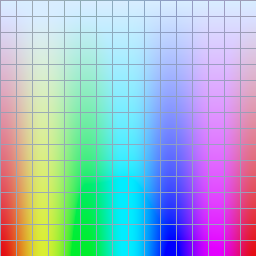
\includegraphics[width=\linewidth]{img/upsampling_texture_original.png}
		\caption{Original\\ }
		\label{fig:sigUpliftOriginal}
	\end{subfigure} \hspace{0.1em}
	\begin{subfigure}[t]{0.22\textwidth}
		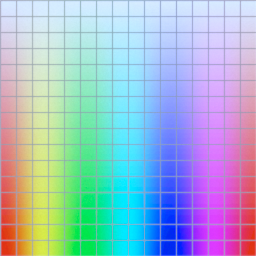
\includegraphics[width=\linewidth]{img/upsampling_texture_copyNeighbor.png}
		\caption{Nearest\\Neighbor}
		\label{fig:sigUpliftNearestNeighbor}
	\end{subfigure} \hspace{0.1em}
	\begin{subfigure}[t]{0.22\textwidth}
		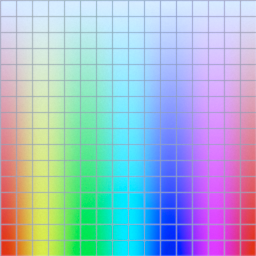
\includegraphics[width=\linewidth]{img/upsampling_texture_interpCoeff.png}
		\caption{Interpolated\\Coefficients}
		\label{fig:sigUpliftInterpCoeff}
	\end{subfigure} \hspace{0.1em}
	\begin{subfigure}[t]{0.22\textwidth}
		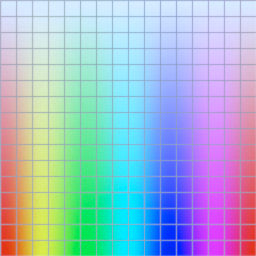
\includegraphics[width=\linewidth]{img/upsampling_texture_interpSpectra.png}
		\caption{Interpolated\\Spectra}
		\label{fig:sigUpliftInterpSpectra}
	\end{subfigure}
	\vspace{0.5em}\\
	\begin{subfigure}[t]{0.22\textwidth}
		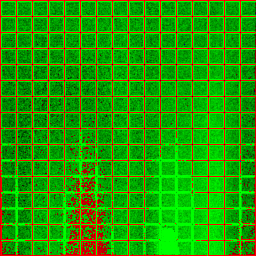
\includegraphics[width=\linewidth]{img/uplifting_diff_originalNeighbor.png}
		\caption{Original\\vs\\Nearest Neighbor}
		\label{fig:sigDiffOrigNeighbor}
	\end{subfigure} \hspace{0.1em}
	\begin{subfigure}[t]{0.22\textwidth}
		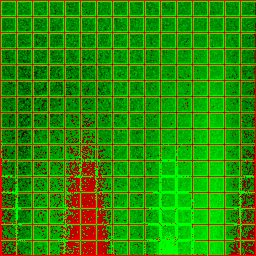
\includegraphics[width=\linewidth]{img/uplifting_diff_originalSpectra.png}
		\caption{Original\\vs\\Interp. Spectra}
		\label{fig:sigDiffOrigSpectra}
	\end{subfigure}\hspace{0.1em}
	\begin{subfigure}[t]{0.22\textwidth}
		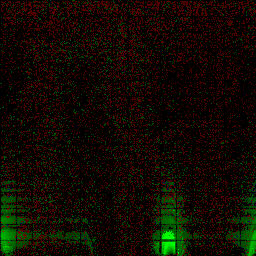
\includegraphics[width=\linewidth]{img/uplifting_diff_spectraCoeffs.png}
		\caption{Interp. Spectra\\vs\\Interp. Coefficients}
		\label{fig:sigDiffSpectraCoeffs}
	\end{subfigure} \hspace{0.1em}
	\begin{subfigure}[t]{0.22\textwidth}
		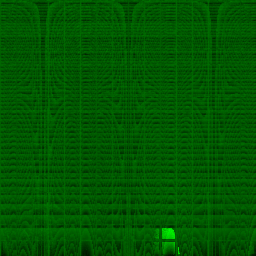
\includegraphics[width=\linewidth]{img/uplifting_diff_spectraNeighbor.png}
		\caption{Interp. Spectra\\vs.\\Nearest Neighbor}
		\label{fig:sigDiffSpectraNeighbor}
	\end{subfigure}
	\caption{Comparison of techniques for obtaining spectra for arbitrary colors in the RGB cube. a) shows the original texture (converted from .exr), while b), c) and d) are rendered with ART by uplifting the texture to its spectral version. All the other figures show differences between some of the pairs. The exposure of the e), f) and h) difference images is increased to 3 for the errors to be visible, and the exposure of the g) image is increased to almost 7.}
	\label{fig:sigmoidTexture}
\end{figure}

An obvious case in which it is possible to avoid any kind of interpolation or approximation is when the RGB values that will be required during the uplift are known beforehand. They can then be added as lattice points to the RGB cube. This is especially useful when attempting to uplift specific textures or materials, which is, in fact, what this method was originally intended for.

This uplifting model is, in many cases, superior to the ones already mentioned above. First of all, the round-trip error yields 0 in the sRGB gamut. In other gamuts within the spectral locus, it outperforms other models as well. Moreover, the execution speed is by far the best, even with the uplifting process running beforehand. 

The smoothness of the spectra can be considered both an advantage and a limitation. Although such spectra closely resemble real-life spectra and are suitable for the interpolation process, they cannot describe extremely bright and saturated spectra, as these tend to be more blocky.

The approach by~\citet{upsamplingFluorescence} tries to solve this issue by extending the set of three sigmoid coefficients with three additional ones specifically designed for handling fluorescence. Its goal is to avoid creating blocky spectra at gamut boundaries and rather create smooth spectra with added fluorescent dyes to compensate for the lack of saturation. Similarly to~\citet{upsamplingJakobHanika}, the uplifting model is also based on an RGB cube structure optimized by the CERES solver. It is expected for the optimization to take longer, as it has 6 coefficients to consider. However, the method is the first one capable of simulating fluorescent spectra, which is especially useful for wide-gamut input textures. 

The problem arising with a requirement to uplift RGB values that do not have a mapping, which we discussed in the previous approach, is solved differently in this case. As both the nearest neighbor and interpolation of coefficients do not produce satisfactory results, \emph{reradiation matrices} of the neighbor lattice points are used. Although this leads to higher memory requirements, the results are smoother and do not produce disruptive artifacts. 

In this section, we have presented multiple techniques capable of spectral uplifting. They differ in numerous aspects --- the round-trip error, execution time, the gamut they are capable of uplifting, whether all uplifting constraints are satisfied, etc. However, the aspect we focus on most in this thesis is the shape of the uplifted spectra, which further affects the color's behavior during rendering, especially under various illuminants. We show a comparison of spectral shapes created by different techniques by uplifting the same RGB value in~\cref{fig:upliftingTechniques}.

\begin{figure}[t!]
	\centering
	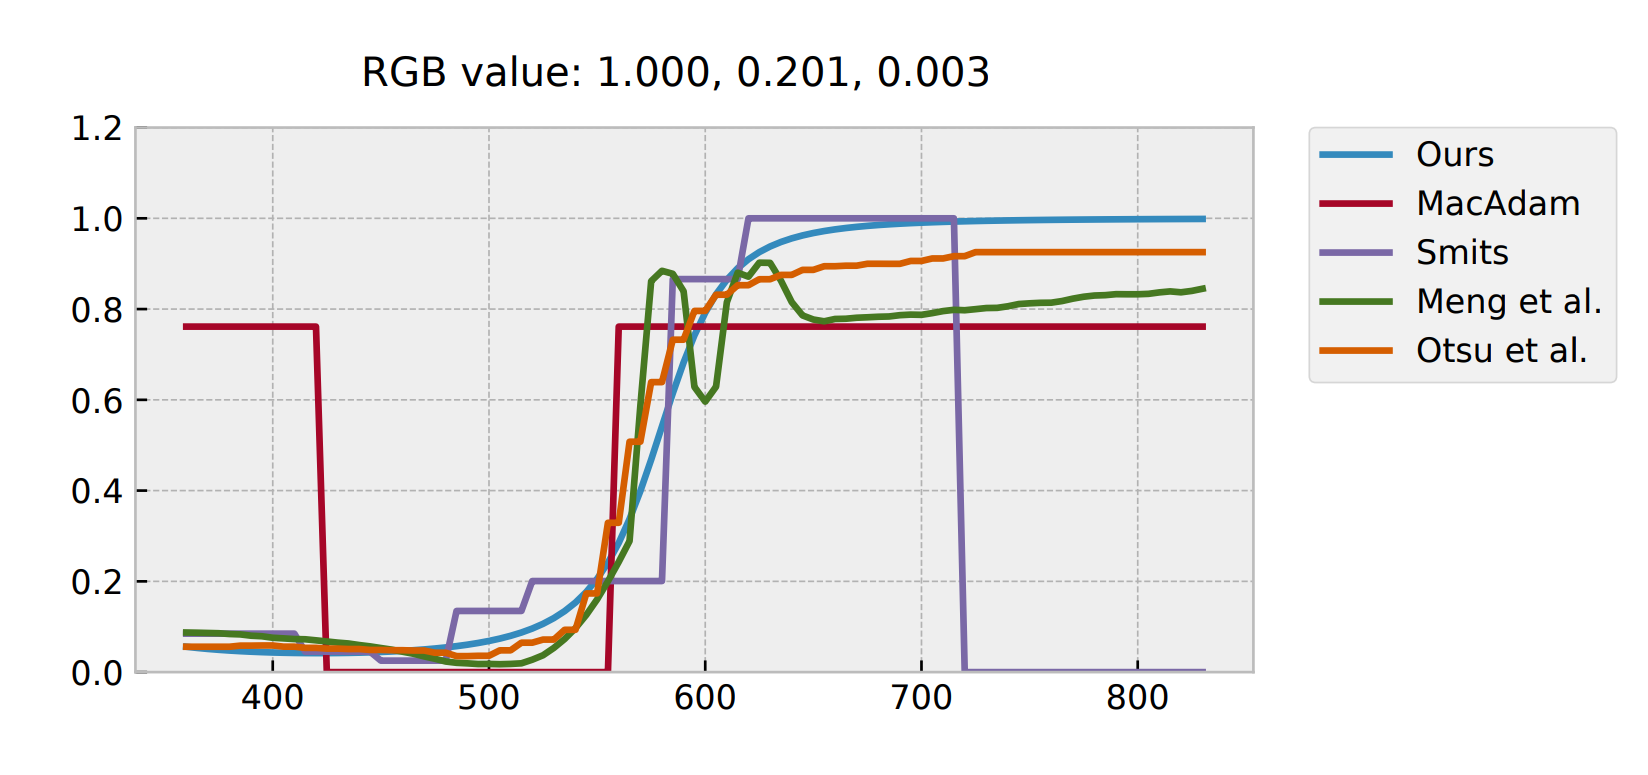
\includegraphics[width=0.8\linewidth]{img/upsampling_techniques.png}
	\caption{Comparison of spectral uplifting techniques as shown by~\citet{upsamplingJakobHanika}. All spectra were created by uplifting the (1, 0.201, 0.003) RGB value and the results were plotted according to the corresponding techniques. The ``Ours'' approach, in this case, refers to the approach by~\citet{upsamplingJakobHanika}.}
	\label{fig:upliftingTechniques}
\end{figure}

\section{Constrained spectral uplifting}

Achieving identity of our uplifted spectra to the real-world spectra is, obviously, impossible. However, uplifting many RGB-based models does not require us to be able to uplift the whole RGB gamut, but only the color spectrum used for the creation of said models. As it is pretty common for the artists in the VFX modeling industry to use specific color atlases when designing textures and materials, the ability to \emph{constrain} the uplifting system with these base colors would be extremely useful in such cases.

In other words, the user would define specific RGB:spectra mappings which would later be used in order to uplift certain RGB triplets. RGB values that would not have a pre-defined mapping would be uplifted by altering the curves of their already-mapped neighbors. 

We call this process \emph{constrained spectral uplifting}. The fact that it does not provide as much freedom as other spectral uplifting approaches works for our benefit, as the results are not a subject to high metamerism, which is, after all, the goal of this thesis.

In this thesis, we base the algorithm used to implement constrained spectral uplifting on~\cref{alg:upliftingAlgSigmoid}. We also use an RGB cube as a structure for saving the mappings, and we also create an uplifting model before rendering. We leave the specific details of implementation to ref. In this section, we discuss the theoretical background of the constraining itself. Specifically, we focus on the means of storing the individual spectra in our structure and the problems that arise along with it.

\subsection{Spectral sampling}

The constraining process starts when the user inserts a set of spectra. Finding an RGB match and creating a mapping is a straightforward task --- one must simply convert the spectra to RGB. However, the spectra must then be stored in the structure, which requires its discretization.

As the spectra must already be discretized on the input by the user (e.g. each spectrum can be defined in a form of an array which specifies reflectance values in 1nm intervals, starting from 380nm), the first approach that comes to mind is to simply store its every ith value. However, for a good color reproduction, around 30 samples are needed for each spectrum~\cite{trigonometricMomentsPresentation}. Storing so many values is extremely memory inefficient, especially when taking into account all the other mappings that must be created later in the system.

Another issue with such storage arises during the approximation stage of the uplifting process. Trying to approximate so many values is infeasible for any optimizer. We must therefore create a more compact representation, which recreates the spectra as efficiently as possible.

We have already talked about approaches to spectral uplifting in~\cref{sec:upliftingMethods}. However, all of them were concerned with the opposite problem --- how to create \emph{any} kind of spectra that evaluates to a specific RGB value. They are therefore restricted to a concrete spectral space and unable to recreate every possible curve. We see an example of this in~\cref{fig:specRecUpliftingMethods}, where the resulting spectra of the uplifting process of multiple methods are compared to the actual measured spectrum of the real-life material.

The simple and smooth shape of the spectra indicate that using a lower-dimensional linear function space, such as Fourier series, could be the key to their storage. Techniques based on this observation have been studied for the storage of emission spectra~\cite{fourierRepresEmission}, and appear promising also for reflectance spectra. This method is studied in an article and subsequent presentation by~\citet{trigonometricMomentsPresentation}. As the reflectance spectra are aperiodic, it is reasonable for the Fourier basis to consist of cosine transforms only. Eventually, a truncated Fourier series is used for the reconstruction, which is computed according to the following equation:
\begin{equation} \label{truncatedFourierSeries}
  f = \sum_{i=0}^{m}c_j cos(j\varphi)
\end{equation}
where $c_j$ are the Fourier coefficients eventually stored in the RGB cube.

We show an example of a result obtained by this method in~\cref{fig:specRecTruncatedFourier}. Although the reconstruction is not far off, the resulting spectra do not always have a physical counterpart, as the reconstruction does not obey the (0,1) reflectance range constrain. We can see this behavior even in our example in~\cref{fig:specRecTruncatedFourier}.

\begin{figure}[t]
	\centering
	\begin{subfigure}[t]{0.45\textwidth}
		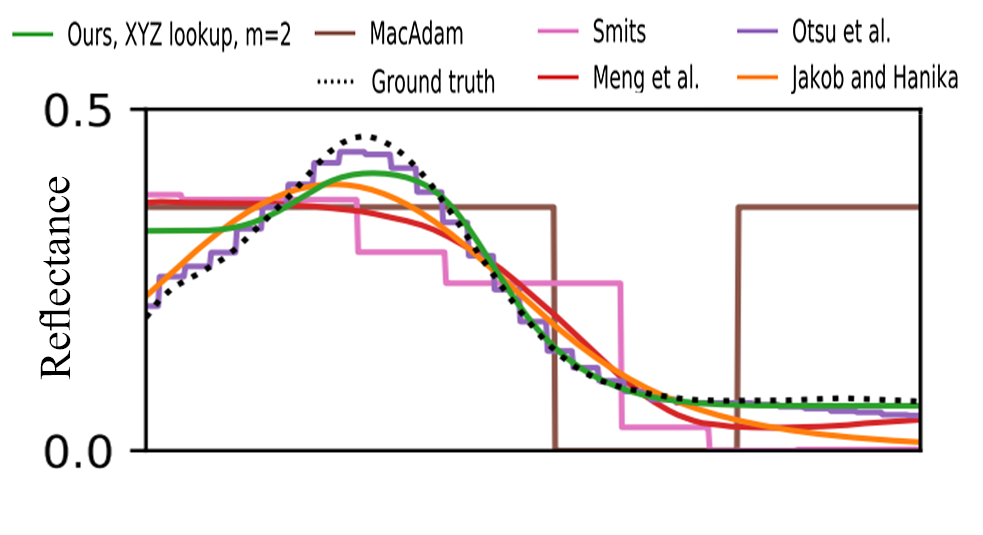
\includegraphics[width=\linewidth]{img/spectra_rec_method_comparison.png}
		\caption{Reconstruction with uplifting models as plotted by~\citet{trigonometricMomentsPaper}, where \emph{Ours} represents a newly proposed technique}
		\label{fig:specRecUpliftingMethods}
	\end{subfigure} \hspace{0.1em}
	\begin{subfigure}[t]{0.45\textwidth}
		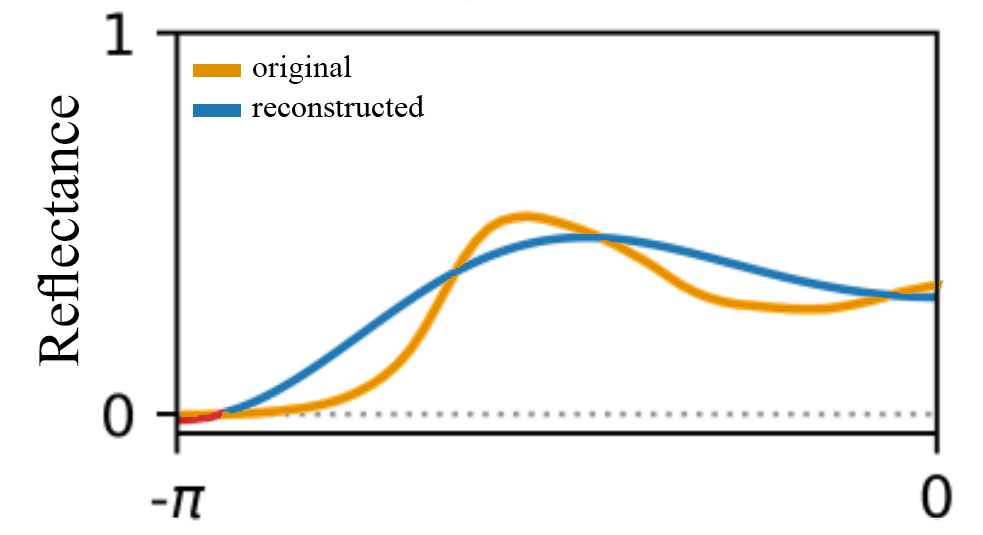
\includegraphics[width=\linewidth]{img/spectra_rec_truncated_fourier.png}
		\caption{Reconstruction with truncated Fourier series~\cite{trigonometricMomentsPresentation}}
		\label{fig:specRecTruncatedFourier}
	\end{subfigure}
	\caption{Comparison of real-life measured spectra and a few techniques that aim for reconstruction of this spectra.}
	\label{fig:spectraReconstruction}
\end{figure}

In contrast to linear function space, spectra can also be represented non-linearly. These representations are, however, incompatible with linear prefiltering of textures~\cite{trigonometricMomentsPaper}.

Therefore, a novel approach has been proposed by~\citet{trigonometricMomentsPaper} in order to eliminate the flaws of both linear and non-linear approaches. In contrast, it utilizes the strengths of these approaches --- the representation consists of Fourier coefficients (which implies compatibility with linear filtering), and the reconstruction is non-linear, based on the theory of moments, and aims for the (0,1) range constraint satisfaction.

Following, we provide a brief overview of both the algorithm for obtaining coefficients and the reconstruction process. For more details, we refer the interested reader to the original article~\cite{trigonometricMomentsPaper}.

\paragraph{Obtaining coefficients} \label{par:spectrumToCoefficientConversion}

The first problem with obtaining the coefficients is caused by the shape of the spectra. In contrast to the Fourier basis, they are aperiodic. Their storage with Fourier coefficients therefore requires their conversion to a periodic signal.

Wavelengths can be mapped linearly to a $2\pi$-periodic signal. This, however, causes distortions and strong artifacts at the boundaries. Moreover, Fourier coefficients computed for such signal are complex, which requires almost twice the memory for storage.

These problems can be solved by mapping only the negative values of the signal as in the following equation:
\begin{equation} \label{wavelengthPhaseMapping}
\varphi =\pi \dfrac{\lambda - \lambda_{min}}{\lambda_{max} - \lambda_{min}} - \pi\in[-\pi, 0]
\end{equation}

By mirroring the signal for the positive part, i.e. defining the resulting mapping as $g(\varphi) = g(-\varphi)$ for all $\varphi\in[0,\pi]$, we get smooth transitions at boundaries. The Fourier coefficients are then computed only from this mirrored signal and the reconstruction also uses only that part of the signal. Although this might seem wasteful, the signal created by this approach is even and therefore requires only real Fourier coefficients for its representation, which benefits the storage requirements. We call this approach to the mapping \emph{mirroring}.

Another proposed improvement to obtaining the coefficients is focusing accuracy on important regions, also called \emph{warping}. This is achieved by means of a differentiable, bijective function that maps the wavelength range to the $[-\pi, 0]$ and is used as a weighting function when computing coefficients. This is useful especially when using only small number of coefficients that are unable to capture more complex curves.

Note that using $m$ complex Fourier coefficients for storing a spectrum implies that that $m+1$ coefficients are actually saved. The $+1$ factor stands for the zeroth moment $c_0$, which is real in both the mirrored and the non-mirrored case. Therefore, overall, mirroring requires storing $m+1$ scalars, while non-mirroring requires $2m+1$ scalars.

\paragraph{Reconstruction} 

The default Fourier coefficients (without improvements such as mirroring and warping) are stored for a $2\pi$-periodic signal $d(\varphi)$, where $d(\varphi) \ge 0$ is a density for all phases $\varphi \in \R$. Therefore, they satisfy the definition of trigonometric coefficients for the \emph{trigonometric moment problem}~\cite{trigonometricMomentProblemDefiniton}. Specifically, the coefficients $\gamma$ can be expressed as
\begin{equation} \label{trigonometricCoeffsComputation}
\gamma = \int_{-\pi}^{\pi} d(\varphi) c(\varphi)d_\varphi \in C^{m+1},
\end{equation}
where $d(\varphi)$ is the finite measure that they represent, and $c(\varphi)$ is the Fourier basis.

By building upon this observation, the reconstruction of spectra is based on the theory of moments, specifically on Maximum Entropy Spectral Estimate (MESE)~\cite{unboundedMESEoriginal}. The MESE has been shown to produce impressive results when used for the reconstruction of emission spectra, as it is capable of reconstructing both smooth and spiky spectra.

However, the problem with this approach is that it is not bounded, i.e. not suitable for reflectance spectra. Therefore, a novel, \emph{bounded MESE}, is introduced. It is based on the research by~\citet{dualityBoundedUnboundedMarkoff} and, subsequently,~\citet{dualityBoundedUnboundedKrein}, who developed a duality between bounded and unbounded moment problems formulated in terms of Herglotz transform. This duality is used for transforming trigonometric moments to \emph{exponential moments} so that the bounded problem represented by the trigonometric moments has a solution if and only if the dual unbounded problem represented by the exponential moments has a solution.

The summary of the reconstruction process is as follows:
\begin{enumerate}
	\item compute exponential moments from the trigonometric moments
	\item evaluate unbounded MESE for the exponential moments
	\item compute bounded MESE by applying duality to the unbounded MESE
\end{enumerate}

The results of the spectral reconstruction itself are impressive, especially when applied to smooth reflectance spectra. We show some examples of this in~\cref{fig:momentsReconstructionPeters}. Even with small number of parameters ($m=3$), the reconstruction describes the original curve quite accurately. Obviously, increasing the number of moments implies higher accuracy, however, it is not recommended to use over 15 moments, as that is roughly the boundary where the mean error stabilizes and does not improve much from then on. Moreover, it is recommended to always use warp for $m \le 5$.

\begin{figure}[t]
	\centering
	\begin{subfigure}[t]{0.70\textwidth}
	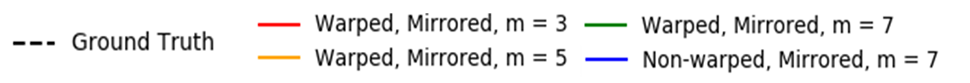
\includegraphics[width=\linewidth]{img/moments_reconstruction_legend.png}
	\end{subfigure} \\
	\vspace{1em}
	\begin{subfigure}[t]{0.45\textwidth}
		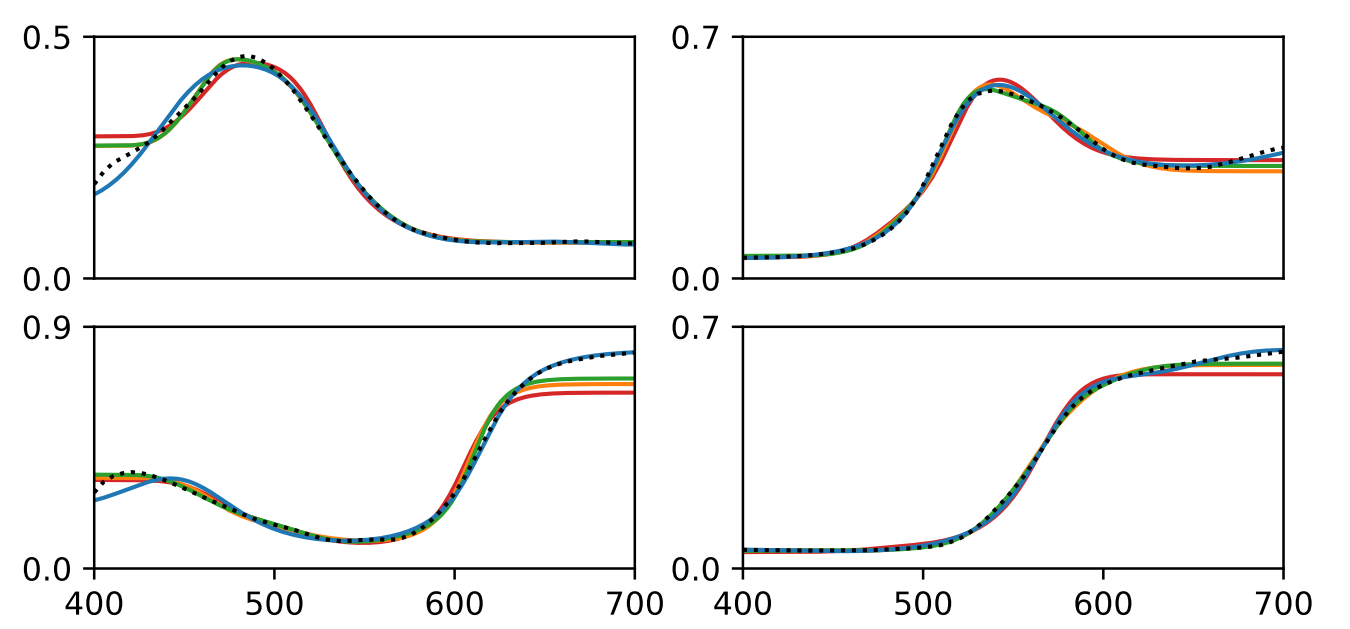
\includegraphics[width=\linewidth,height=0.2\textheight]{img/moments_reconstruction_Peters.png}
		\caption{Examples of reconstruction of smooth spectra as provided by~\citet{trigonometricMomentsPaper}.}
		\label{fig:momentsReconstructionPeters}
	\end{subfigure} \hspace{0.1em}
	\begin{subfigure}[t]{0.45\textwidth}
		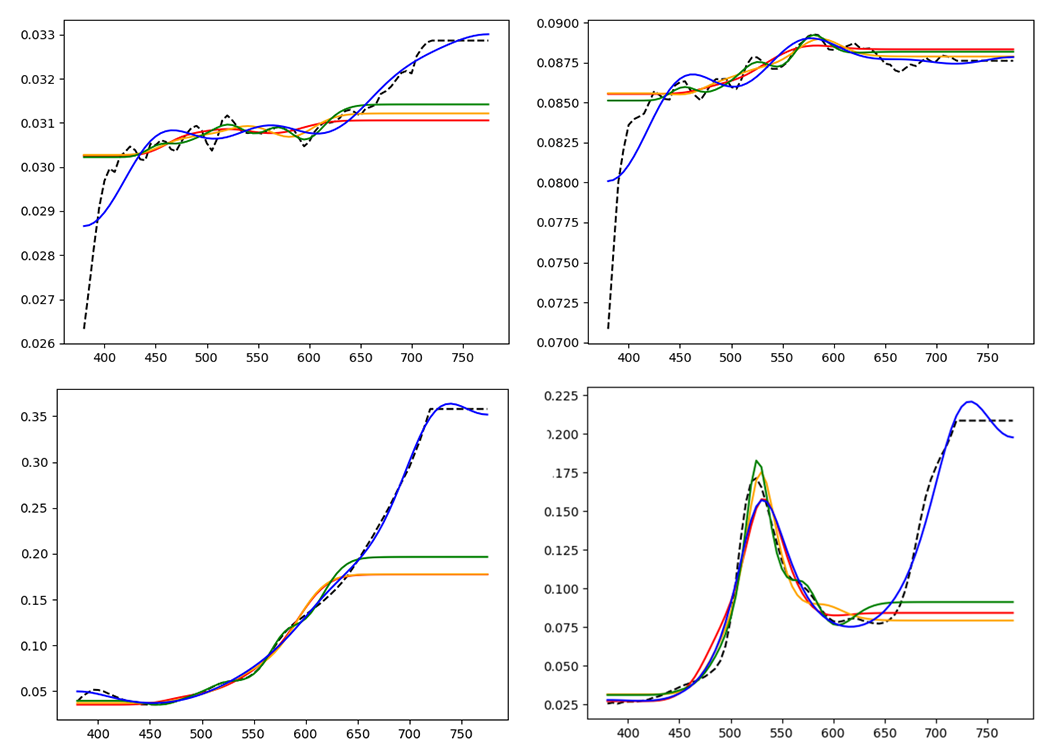
\includegraphics[width=\linewidth]{img/moments_reconstruction_ours.png}
		\caption{Reconstruction of spectra of the Macbeth chart as plotted by us. Top left: ``black'' patch; top right ``neutral35'' patch; bottom left: ``dark skin'' patch; bottom right: ``foliage'' patch.}
		\label{fig:momentsReconstructionOur}
	\end{subfigure}
	\caption{Examples of reconstruction with the trigonometric moment method.}
	\label{fig:momentsReconstructionComparison}
\end{figure}

This technique can also be used for the storage of emission spectra. As these tend to be more spiky and sharp, a lot more moments is required than for the reflectance spectra. To give an example, even a mirrored approached with $m=15$ does not produce satisfactory results for some emission spectra and the testing was performed for as many as real 32 moments ($m=31$). Even then, the approach was unable to reconstruct some details.

In this thesis, we focus on storing reflectance spectra. However, in contrast to the spectra shown in~\cref{fig:momentsReconstructionPeters}, we expect some of our to not be so smooth and to have sharper edges. We show examples of such spectra in~\cref{fig:momentsReconstructionOur}, where we also attempt to save and reconstruct them in the same manner as shown in~\cref{fig:momentsReconstructionPeters}. However, the results are not as accurate, which implies the need for more moments.

The number of coefficients that needs to be used depends on many factors, such as the shape of our spectra, available memory and the accuracy for which we aim. We discuss this thoroughly in ref, where we determine the optimal number of coefficients and the method of storing them for our specific problem.

Interpolation of coefficients. Peters hovoria ze by sa mali dat interpolovat, treba spravit experimenty.

Adding a few unimportant words for now, just to see how the images will be aligned when a new paragraph will be added Adding a few unimportant words for now, just to see how the images will be aligned when a new paragraph will be added


\chapter{Implementation}

We approach the problem of spectral uplifting similarly to~\citet{upsamplingJakobHanika}, where an uplifting model is created prior to rendering. Our implementation therefore consists of two parts --- \emph{model creation} and its subsequent \emph{utilization} in a rendering software. 

For the first part, we extend an already existing uplifting tool, the \emph{Borgtool}, which is currently used for creating sigmoid-based RGB cubes as in~\cref{alg:upliftingAlgSigmoid}. We add the possibility for creating trigonometric moment-based cubes, i.e. for the spectra to be stored with trigonometric moments rather than sigmoid coefficients. We also add an option for constraining such a cube with a user-specified atlas.

We then show the performance of such a model by integrating it in ART, which, up until now, used only one built-in sigmoid-based cube for all its uplifting processes.

\section{Uplifting model}

The core of this section is the already mentioned Borgtool. It is a stand-alone, non-open source thing that was created by Weta and is blabla. (spytat sa?)

Currently, the output of the Borgtool is an RGB cube structure which contains multiple entries in form of lattice points. Following, we name the main parameters of a single cube entry:
\begin{itemize}
	\item \emph{target RGB} --- the actual RGB that the point has in the cube.
	\item \emph{coefficients} -- -the sigmoid coefficients used to reconstruct a spectrum so it matches the target RGB.
	\item \emph{lattice RGB} --- the actual RGB that the reconstructed spectrum evaluates to. Ideally, this should match the target RGB.
\end{itemize}
Along with its entries, the resulting cube structure also stores a few other properties, both \emph{static}, such as the illuminant according to which the RGB cube is uplifted, and \emph{user-adjustable}, such as the cube dimension or the fitting threshold (i.e. the maximum allowed difference between the target and the lattice RGB).

Our trigonometric moment-based cube can be viewed as an extension of the sigmoid cube --- in addition to the already existing parameters, we add a user-adjustable \texttt{coefficientCount} variable which specifies the number of coefficients that are to be used for most of the entries, which subsequently requires us to alter the cube entry structure. Furthermore, for the purposes of atlas constraining, we extend the cube entry with an optional pointer to an atlas entry. This is where the main difference between our and the sigmoid cube lies --- while the sigmoid cube regards all of its points as equal, we distinguish between \emph{atlas lattice points}, i.e. the lattice points that correspond to specific atlas entries; and \emph{regular points}, which do not. We place special emphasis on the atlas lattice points, as we require their spectra to be as precise and close to the original spectra as possible. As a result, we choose to always store such spectra with the maximum available coefficients (currently, $9$). Therefore, the \texttt{coefficientCount} variable applies to the regular points only. We explain the reasoning behind this decision and its impact on rendering and overall performance more thoroughly as we continue with this section.

Our uplifting process is also similar to the one already implemented in the Borgtool, which closely follows~\cref{alg:upliftingAlgSigmoid}. Following are the individual steps of the process:
\begin{enumerate}
	\item \emph{Initialization}
	\item \emph{Fitting of starting points}
	\item \emph{Cube fitting}
	\item \emph{Cube improvement}
	\item \emph{Cube storage}
\end{enumerate}

\subsection{Initialization}

This part of the run is responsible for three things:
\begin{itemize}
	\item parsing of the parameters
	\item initialization of the cube and its entries with default values
	\item loading of the required color atlases
\end{itemize}

The initialization of the cube is pretty straightforward, as all of its properties are either user-defined or set to default (note: the default illuminant is always D65). The number of cube entries is directly proportional to the cube's \texttt{dimension} parameter, which specifies the number of entries per one axis. This renders the total number of entries to $dimension^3$. As the lattice points are positioned evenly, their target RGB values are then equivalent to their coordinates in the RGB cube.

The loading of the atlases is a bit more complicated. Firstly, a single color atlas is inputted in a form of a simple .txt file, which contains merely a list of entries in a textual form as shown in~\cref{fig:macbethSampleText}. Therefore, it requires parsing.

\begin{figure}[t]
	\lstset{
		string=[s]{"}{"},
		comment=[l]{:},
		commentstyle=\color{black},
		basicstyle=\scriptsize
	}
	\begin{lstlisting}
Entry ID:   orange
---------------------------------------------------------------------------
Description           :  "orange" patch of the Macbeth colour checker
Type                  :  reflectance spectrum
Fluorescence data     :  no
Measurement device    :  
Measured by           :  
Measurement date      :  

Sampling information
--------------------
Type	    	      :  regular
Start                 :  380.0 nm
Increment             :  5.0 nm
Maximum sample value  :  100.0

ASCII sample data
-----------------
{6.143748,  5.192119,  4.867970,  5.092529,  4.717562,  4.663087,  4.455331,  4.562958,  4.517197,  4.536289,  4.454180,  4.543101,  4.491708, ... }

	\end{lstlisting}
	\caption{A sample entry from the Macbeth Color Checker atlas.}
	\label{fig:macbethSampleText}
\end{figure}

Moreover, the spectral data obtained from the atlases cannot be stored in the Borgtool directly, so as to avoid extreme memory requirements arising with large atlases. To solve this problem, we take advantage of the trigonometric moments.

We store the spectral curves of the individual atlas entries by using the Fourier coefficients as described in~\cref{par:spectrumToCoefficientConversion}. We use the maximum number of available moments (currently 9, see explanation in~\cref{ssec:ceresSolver}), and we both mirror and warp the signal prior to coefficient computation. We explain the reasoning behind this in~\cref{sec:storingMoments}, where we run experiments to decide on the most efficient and precise method.

\subsection{Fitting of starting points}

In order to uplift the whole cube as described in~\cref{alg:upliftingAlgSigmoid}, we must first fit one or more \emph{starting points} whose coefficients can then be used as prior for the fitting of other lattice points.

For these purposes, we utilize the user-specified color atlas. Ideally, every entry of the color atlas should correspond to one lattice point. We try to achieve this by iterating over the atlas entries, finding the cube voxel in which the current entry should reside in terms of RGB and then choosing the closest lattice point from all 8 corners of the voxel. We classify this lattice point as an \emph{atlas lattice point} and we assign it the coefficients saved for the current atlas entry. We call this process the \emph{seeding} of the cube.

Obviously, achieving a complete injection between atlas entries and their respective lattice points is not always possible. In some cases, we might find that the closest lattice point to an atlas entry we are about to map has already been seeded. This might be due to the following reasons:
\begin{itemize}
	\item the number of atlas entries is higher than the size of the cube
	\item the atlas entries are concentrated around specific colors (e.g. we seed a very small cube with only the Page 14 from the Munsell Book of Colors as in ukazka)
\end{itemize}
In both cases, we issue a warning and recommend the user to use a higher dimensional cube.

By seeding the cube, we have appointed coefficients to some of the lattice points. These coefficients reconstruct a spectrum that evaluates to an RGB value which we denote as the \emph{lattice RGB}. The difference between the lattice and the target RGB is therefore equal to the distance between the lattice point and its assigned atlas entry. It is apparent that the distance may be higher than the defined fitting threshold. In such cases, we must ``improve'' upon the coefficients so that the resulting color difference is as low as possible.

Our problem of improving the coefficients satisfies the definition of the \emph{Non-linear Least Squares} problem~\cite{nonLinearLeastSquares}. Non-linear Least Squares is an unconstrained minimization problem in the following form:
\begin{equation} \label{eq:nonLinearLeastSquares}
	 \underset{x}{\text{minimize}} \hspace{0.5em} f(x) = \sum_{i} f_{i}(x)^{2},
\end{equation}
where $x= \{x_{0}, x_{1}, x_{2}, ... \}$ is a parameter block that we are trying to improve (i.e. our coefficients) and $f_{i}$ are so-called \emph{cost functions}. The definition of cost functions is dependant solely on the current problem. In our case, we primarily require to minimize the difference between the lattice and the target RGB. Our secondary requirement is the shape similarity of the original atlas entry curve and the resulting curve of the atlas lattice point. This gives rise to multiple choices for cost functions, such as using the difference between curves along with the Delta E error, using one or multiple cost functions for the RGB error etc\ldots After implementing some of them and testing their performance, the results of which we provide in ref, we decide on neglecting the shape similarity requirement and using three cost functions, each specifying the absolute difference in one of the three axes of the cube.

To solve an optimization problem defined in such a way, we use the CERES solver.

\subsubsection{CERES solver} \label{ssec:ceresSolver}

As already mentioned in~\cref{sec:upliftingMethods}, the CERES solver is an open-source library for solving large optimization problems such as our Non-linear Least Squares problem. It consists of two parts --- a \emph{modeling API} which provides tools for the construction of optimization problems, allowing us to set parameters such as maximum number of iterations of the optimizer and maximum number of consecutive nonmononotic steps; and a \emph{solver API} that controls the minimization algorithm.

To solve a Non-linear Least Squares problem, the solver requires us to specify only a so-called \emph{residual block}, which is a structure defined by the prior coefficients and the cost functions. During the execution, the solver tries to minimize the values of the cost functions (or \emph{residuals}) in the residual block. The execution is aborted and the current best parameter block returned when the solver achieves either the specified number of iterations or nonmonotonic steps. For more information on the specifics of the CERES solver, we refer the interested reader to its documentation by~\citet{ceresNonLinearLeastSquares}.

There are two main downsides to using the CERES solver. Firstly, the maximum allowed size for a parameter block when using a numeric cost function is 9. This means that we are not able to use more than 9 coefficients for storing a spectrum. This issue could be resolved by adding more residual blocks and combining their results. However, as the runtime of both fitting and rendering with 9 coefficients is already substantially high, we decide not to add such an option as it would most likely be unused.

Another, greater issue is the possibility of CERES getting stuck in local minima and therefore produce unsatisfactory results. This may happen due to the following reasons:
\begin{itemize} \label{ceresDeficiency}
	\item the dimension of the cube is too low, i.e. the prior coefficients are extremely distinct from the ideal coefficients, or
	\item the number of coefficients is too high, i.e. the optimizer fails in improving them as a whole
\end{itemize}
In such cases, the optimizer is not capable of leaving the local minima on its own. We therefore apply a simple heuristics, which consists of only slightly altering the first coefficient (or the first and the second) and running the optimizer again. We chose to alter the first coefficients because they influence the shape of the curve the most.

The need for a heuristic suggests considerable difference between the prior and the resulting coefficients, which implies distinct spectral curves. Such a behavior is undesired, as it may result in strong metameric artifacts. Fortunately, this heuristic is rarely triggered. We examine this in ref, where we analyze the success rate of the fitting and also demonstrate the curve differences by showing both the spectral curves of the atlas entries and of the fitted lattice points.

The sigmoid-based method approaches the starting points problem by selecting the point in the center of the cube and initializing its coefficients to zero. As these values are extremely close to the real values of coefficients, the optimizer does not have a problem with the fitting.

We inspire ourselves by this approach and provide an option for starting in the middle as well. This eliminates the obligation of the user to specify an atlas, i.e. if no atlas is specified, the cube is fitted from the center. However, providing such an option requires us to define a set of prior coefficients for the center point. We determine it by iterating over multiple existing color atlases and searching for spectral curves that roughly evaluate to an RGB of $(0.5, 0.5, 0.5)$. The coefficients of such curves are roughly $\{0.5, 0, 0, 0, ... \}$, i.e. all zeroes except for the first coefficient. We use these prior coefficients for all available moments and cube dimensions.

\subsection{Cube fitting}
Once the starting points are successfully fitted, we can use their coefficients as prior for other lattice points. We proceed similarly to the approach in~\cref{alg:upliftingAlgSigmoid}, where the lattice points are fitted in multiple \emph{fitting rounds}, each round attempting to fit the neighbors of the already fitted points. We provide a more detailed description of the principle behind our fitting algorithm in~\cref{alg:upliftingAlgMoments}.

\begin{algorithm}[t!]
	\caption{Fitting of the cube from starting points}
	\label{alg:upliftingAlgMoments}
	\begin{algorithmic}[1]
		\State $n \gets $ user-defined number of coefficients
		\State $fittingRound \gets$ $0$
		\State $unfittedPoints \gets$ a list of all points in $RGBCube \setminus startingPoints$
		\ForAll{$point \in unfittedPoints$}
		\State $point.fittingDistance = MAX\_DOUBLE$
		\EndFor
		\While {$unfittedPoints$ is not empty}
		\State{$currRoundPts \gets$ points from $unfittedPoints$ that have at least one fitted neighbor}
		\ForAll{$point \in currRoundPts$}
		\ForAll{$fittedNeigbor \in point.neighbors$}
		\State $point.coefs \gets fittedNeighbor.coefs$
		\If{$fittedNeighbor \in atlasLatticePoint$} \label{algStep:conversionBegin}
		\State{$spectrum \gets$ reconstruct spectrum from $fittedNeighbor.coefs$}	
		\State{$fittedNeighbor.coefs \gets$ save $spectrum$ with $n$ coefficients} \label{algStep:conversionEnd}
		\EndIf 
		\State $currDistance \gets $ CERES.Solve($point.coefs$, $costFunctions$)
		\If{$currDistance \leq point.fittingDistance$} \label{algStep:improvementStart}
		\State $point.fittingDistance \gets currDistance$
		\State $point.coefs \gets $ coefficients from solver
		\EndIf
		\If{$currDistance \leq fittingThreshold$}
		\State break
		\EndIf \label{algStep:improvementEnd}
		\EndFor
		\While{$point.fittingDistance > fittingThreshold$} \label{algStep:heuristicsStart}
		\State use heuristics to improve upon the current coefficients
		\State run the solver again
		\State repeat steps \ref{algStep:improvementStart} $-$ \ref{algStep:improvementEnd}
		\If{too many iterations of the while cycle have been performed}
		\State break \label{algStep:heuristicsEnd}
		\EndIf
		\EndWhile
		\If{$point.fittingDistance > fittingThreshold$}
		\State remove $point$ from $unfittedPoints$
		\EndIf
		\If{$point$ has tried the coefficients of all of its neighbors}
		\State remove $point$ from $unfittedPoints$
		\EndIf
		\EndFor	
		\State $fittingRound \gets fittingRound+1$
		\EndWhile
	\end{algorithmic}
\end{algorithm}

Similarly to the cube structure, our algorithm also extends the implementation provided in the sigmoid fitting. Two main features are added --- conversion of coefficient representation (i.e. \emph{coefficient recalculation}) and an improvement heuristic.

\paragraph{Coefficient recalculation}

Up until now, all the uplifting techniques mentioned used the same number of coefficients per lattice point. The reasons for this were both consistency of the representation and the possibility of coefficient interpolation. The latter is especially useful in rendering, as interpolation of coefficients instead of whole spectra substantially increases performance.

We, however, chose to use a different number of coefficients for atlas lattice points and regular points. Although this might sound counter-intuitive, we defend our decision by regarding the performance of the optimizer.

As the time execution of the spectral reconstruction is dependant on the number of coefficients, it is evident that by increasing the number of coefficients, we increase the time requirements of the optimizer. Additonaly, having more coefficients implies more possibilities for the optimizer, which subsequently suggests the need for more iterations. This decreases performance even further.

This does not pose a significant problem when fitting atlas lattice points only, as they usually make up only a small portion of the cube's entries. However, if we were to fit the whole cube with the maximum number of coefficients, we would find a noticeable performance decrease as opposed to fitting with, say, 3 coefficients.

If we therefore wish to preserve representation consistency, we need to either accept the high time execution or give up the precision with which we fit atlas entries. The latter is not a realistic option, as the precise atlas fitting is the ultimate goal of this thesis. The increased time execution is similarly unfeasible, as it takes a lot more time. Furthermore, having more coefficients provides no real benefits to the resulting spectra (see ref). We therefore trade it off and allow the user to insert his own desired number of moments.

The problem we solve in steps~\ref{algStep:conversionBegin} through~\ref{algStep:conversionEnd} of our algorithm is that arising when using atlas lattice points' coefficients as prior to regular points. By supporting two distinct representations of a cube's entry, we simply cannot use the same 9 coefficients as prior to, for example, a point that only requires 4. Luckily, this is easily solved --- we just add a \emph{recomputation} function which reconstructs the spectra of the prior point and subsequently saves it with the new, lower number of coefficients. Obviously, such a conversion causes significant loss of spectral information. However, as we do not need the regular lattice points' coefficients to evaluate to any specific spectra, this does not need to concern us.

Up until now, we have not mentioned the effect of various numbers of coefficients on the interpolation phase of rendering, specifically on the coefficient interpolation. That is because our implementation, similarly to the sigmoid implementation, does not support this and is rather based on the interpolation of spectra. We explain the reasoning behind this in ref DOROBIT. However, if required, adding support for coefficient interpolation does not pose a problem --- we would only need to utilize the already existing recomputation function. We would need to proceed in the opposite manner as before, when we converted 9-coefficient representations to a smaller number of coefficients. Instead, we would need to convert the regular lattice points to their 9-coefficient representation, so as to preserve the spectral precision of the atlas lattice points.

\paragraph{Improvement heuristic}

To minimize the shortcomings of the optimizer mentioned in~\cref{ceresDeficiency}, we add a heuristic-based improvement of the coefficients, implemented in steps~\ref{algStep:heuristicsStart} through~\ref{algStep:heuristicsEnd}. Its implementation consists of solely slightly changing the first coefficient and running the optimizer again for a pre-defined number of times. In constrast to the heuristics applied when fitting atlas entries, we ommit the changing of the second coefficient completely and we also use significantly less iterations when changing the first coefficient. This is because we do not necessarily require the points to be fitted in the given round. Even if the fitting fails, it may still be successful in the following rounds, where the coefficients of newly fitted neighbors might be used as prior. Additionaly, after the cube fitting is done, we still run an ``improvement'' step for the unsuccessful points. We discuss the specifics of this step in~\cref{ssec:cubeImprovement}.

The number of the fitting rounds depends both on the cube dimension and on the kind of atlas that has been used. If we choose not to input an atlas, the fitted cube ``grows'' from the middle, while seeding with an atlas makes the cube ``grow'' from many places, requiring a lot less round. We show the differences in , where we present the 

Obviously, neither option is better in terms of performance, as the number of fitted points must still be the same. 

\subsection{Cube improvement} \label{ssec:cubeImprovement}

In extreme cases, such as when using too many coefficients to store entries of a cube with either a low dimension or a low fitting threshold, fitting some of the points may be unsuccessful even after applying heuristic improvements. We attempt to solve this by simply iterating over all the already fitted points and using their coefficients as prior for our point. We even apply heuristics similar to the ones used during the fitting of atlas entries. This shows to be useful especially if we have an extremely limited number of sets of prior coefficients, which happens usually if the overall size of the cube is small.

We call this process \emph{cube improvement}. Although the heuristic may seem simple and illogical at first, we must once again zvyraznit that it is aimed solely at the most extreme cases. As a matter of fact, it usually does not even get triggered and, if it does, it is only for a highly problematic point of two. We present the exact statistics in ref.

Obviosuly, improving the points as such has its drawbacks. We do not focus on the time performance, as we mainly want this part to be successful rather than fast. Moreover, as this step runs for a small set of numbers only, the execution time is negligible in comparison to other steps.

The more important issue is the shape of the resulting curve. Using seemingly ``random'' coefficients as prior suggests the resulting curve's shape to be unlike those of its neighbors, which may result in metameric artifacts.


The reason behind using improvement heuristics both during and after fitting is both for improved time performance, i.e. a simple change of coefficients is less time-consuming that the process t

and a more desirable resulting shape of the spectral curves. Cube improvement after fitting is extremely time-consuming in contrast to a simple change in coefficients. Moreover, due to reasons explained in~\cref{ssec:cubeImprovement}, the resulting curve could take a shape dramatically distinct from the shape of its neighbors, which is an undesirable behavior. On the other hand, trying to improve all coefficients during the cube fitting would require a complicated heuristic including a lot of optimizer runs, which might eventually lead to a lowered time performance. We show all of these effects in ref.


multithreaded 

We support from 2-8 moments then, however, we will talk about the number of coefficients (although user inserts moments). From now on we talk about coefficients. We do not support 1 or 2 coefs as they only create rovne ciary which does not reconstruct the color we want.

\subsection{Cube storage}
	
Once the cube is completely fitted, its contents are written to a binary file. As we want the resulting file to be as small as possible, we save only the information crucial for the purposes of rendering. Following, we provide a list of contents of a cube file:
\begin{itemize}
	\item \emph{version}
	\item \emph{features}, i.e. whether the cube contains debug information
	\item \emph{moment flag} --- a flag signifying that the cube is based on trigonometric moments. We extend the sigmoid cube structure with a sigmoid flag for an easier cube recognition in rendering software.
	\item \emph{dimension}
	\item \emph{illuminant} under which the cube has been fitted
	\item \emph{fitting threshold}
	\item for every point, we store:
	\begin{itemize}
		\item \emph{coefficient count}, which gives us information on whether the point is an atlas lattice point or a regular point
		\item \emph{coefficients}
		\item \emph{lattice RGB}
		\item \emph{fitting distance}, i.e. the distance between lattice and target RGB, should be below fitting threshold
		\item in case the debug information is included, the entry also contains:
		\begin{itemize}
			\item \emph{target RGB}
			\item \emph{treated variable}, i.e. in which round was the point fitted. If the variable is equal to $-1$, it means the fitting has failed for this point.
		\end{itemize}
	\end{itemize}
\end{itemize}

If we were to use such a cube for the purposes of rendering, the knowledge of both the entry's treated paramter and its target RGB is unnecessary. The only benefit the treated parameter provides is the capability to issue a warning in case the cube is incomplete. This can, however, also be achieved by spectral reconstruction from the coefficients and the comparison of its RGB to that of the entry's lattice point.

Storing the target RGB variable also provides no irreplaceable advantages. The target RGB of all the lattice points can simply be computed from the cube's dimension parameter, rendering such variables useless.

In addition to the storing of the cube, we also provide a function capable of loading such a cube and initializing its parameters. Borgtool utilizes this function in case the user wants to create a texture from an already existing cube or simply wants to check the correctness of the existing cube's parameters. The code of this function is also used during the integration in a rendering software.

\section{ART integration}

The user can choose the size of the cube etc. Borgtool has the following options, and we implement all of them for our method (except for something)
The borgtool already has the sigmoid method implemented as in algorithm daco
Uses three coefficients, fits from middle, and therefore results are metameric (show picture)
We implement the trigonometric moment method by changing up the code provided by peters
We aim for allowing the user to add a color atlas, however we also provide an option when the user fits from the middle
When fitted from middle, the optimizer works very similarly to the sigmoid method (show pictures)

Also explain the threshold value - it is really important to set it properly and that it affects performance.


 as the interpolation of multiple spiky, non-similar spectra often results in a similarly uneven spectrum susceptible to metameric artifacts. Mention here that we NEED to have smooth spectra and that it is very important for interpolation. We therefore set parameters so that this is possible as this is the key. 

\chapter{Results} \label{chap:results}

In this chapter, we talk about the results. We start of by talking about the results achieved with different parameters during implementation and which we decided to use in the end. We then proceed to evaluate

If we were to assume a single-color image map obtained by spectrally rendering one atlas entry and we were to uplift a pixel of this image map, it would be crucial for its position in the RGB cube to be the closest to a lattice point seeded by the original atlas entry, so as to utilize it during uplifting. Even a slight change in the RGB value of the image map may cause the uplifting to consider different point as primary during interpolation, which could lead to undesired behavior. Additionaly, especially in the cases of a low voxel size (i.e. high cube \texttt{dimension} parameter), such a change could even cause the pixel of the image map to be uplifted in a different voxel than the original atlas entry, which might possibly not utilize the atlas entry at all. As the variance in the RGB value of the resulting image map is inevitable due to the stochastic nature of the spectral rendering process, - navyse daco s tymto spravit

\section{Implementation parameters}

\subsection{Storing moments} \label{sec:storingMoments}

The first thing we analyze is the technique used for storage and subsequent reconstruction of the Fourier coefficients. Specifically, we need to decide how to map wavelengths to a signal from which the coefficients are obtained. As already mentioned in~\cref{par:spectrumToCoefficientConversion}, we have the choice of both \emph{mirroring} and \emph{warping} the signal, which overall creates four options --- using only mirroring, using only warping, using both or using neither, i.e. utilizing the original signal.

To decide which of these options suits our problem the best, we run an experiment in which we compare the original color of a spectral curve with the color of a spectrum obtained by reconstruction from the original curve's coefficients. We use entries from multiple color atlases (such as the Pantone atlas, Munsell Book of Colors and Macbeth Color Checker) and we compute the average and maximum color difference. For these purposes, we use the Delta E error specified in~\cref{deltaE}. Although we state that the Delta 2000 is better, it is not(why? MFO) due to  discontinuities when using gradients

In~\cref{sec:completeMomentError}, we provide all results obtained from these experiments. Note that using $n$ moments requires storing $n+1$ values in case mirroring is used (i.e. the moments are real) and $2n+1$ values otherwise (i.e. the moments are complex). As we are interested in the number of $coefficients$ needed for storage (and for passing to the optimizer) rather than the number of moments, we surmise the contents of~\cref{sec:completeMomentError} in~\cref{table:comparisonMomentTechnique}, where we present the errors according to the number of coefficients.

\begin{table}[t]
	\centering
	\begin{tabular}{crrrrrrrr}
		\toprule
		\multirow{4}{*}{Coefficients} &
		\multicolumn{8}{c}{Methods} \\
		\cmidrule(lr){2-9}
		&\multicolumn{2}{c}{M\&W} &
		\multicolumn{2}{c}{M\&nW} &
		\multicolumn{2}{c}{nM\&W} &
		\multicolumn{2}{c}{nM\&nW}\\
		\cmidrule(lr){2-9}
		& Avg & Max & Avg & Max & Avg & Max & Avg & Max \\
		\cmidrule(lr){1-9}
		1&35.87&114.04&36.2&113.86&35.92&113.97&36.2&113.86\\
		2&21.3&91.19&26.4&99.44&\textemdash&\textemdash&\textemdash&\textemdash\\
		3&1.65&15.09&15.43&68.06&6.54&42.93&13.24&60.23\\
		4&0.86&5.6&9.93&55.67&\textemdash&\textemdash&\textemdash&\textemdash\\
		5&0.54&2.98&4.19&23.53&2.13&17.51&3.7&17.5\\
		6&0.34&2.22&1.19&5.68&\textemdash&\textemdash&\textemdash&\textemdash\\
		7&0.29&2.17&0.77&2.38&1.13&6.87&0.95&5.3\\
		8&0.28&2.03&0.77&1.86&\textemdash&\textemdash&\textemdash&\textemdash\\
		9&0.26&1.95&0.62&1.43&0.97&4.35&0.48&1.96\\
		\bottomrule
	\end{tabular}
	\caption{The average and maximum \emph{Delta E} error originating from round-trips, i.e. from converting spectra to coefficients $c$ and its subsequent reconstruction from $c$. $M$ represents mirroring, $W$ warping, and the symbol $n$ stands for their negation.}
	\label{table:comparisonMomentTechnique}
\end{table}

According to the observation of~\cref{table:comparisonMomentTechnique}, it is clearly beneficial to use mirroring. Choosing whether to warp the signal is slightly more complicated --- warping definitely performs better if the number of coefficients is below six (as a matter of fact, this is exactly the same conclusion that~\citet{trigonometricMomentsPresentation} has arrived to), and on average outperforms the non-warping strategy even when using higher number of coefficients. We, however, require successful round-trips only when fitting atlas lattice points, as the regular points do not have a prior atlas entry that their spectra must approximate. We therefore focus exclusively on the performance of these technique under 9 coefficients, as that is the number we use for fitting such entries. 

\begin{figure}[t]
	\centering
	\captionsetup[subfigure]{font=footnotesize,labelfont=footnotesize}
	\captionsetup[subfigure]{justification=centering}
	\begin{subfigure}[t]{0.60\textwidth}
		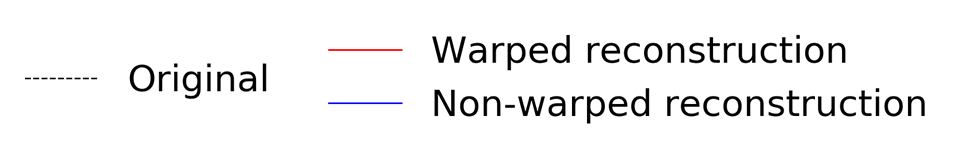
\includegraphics[width=\linewidth]{img/results_techniqueLegend.png}
	\end{subfigure} \\
	\begin{subfigure}[t]{0.45\textwidth}
		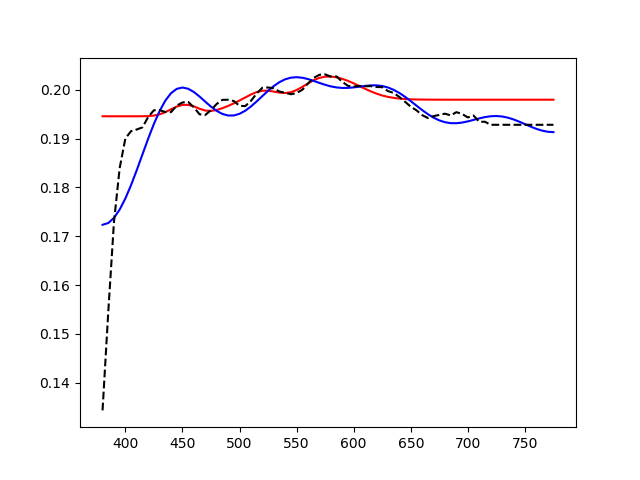
\includegraphics[width=\linewidth]{img/results_techniqueNeutral5.png}
		\caption{``neutral 5'' patch}
		\label{fig:resultsTechnique_neutral5}
	\end{subfigure} \hspace{0.1em}
	\begin{subfigure}[t]{0.45\textwidth}
		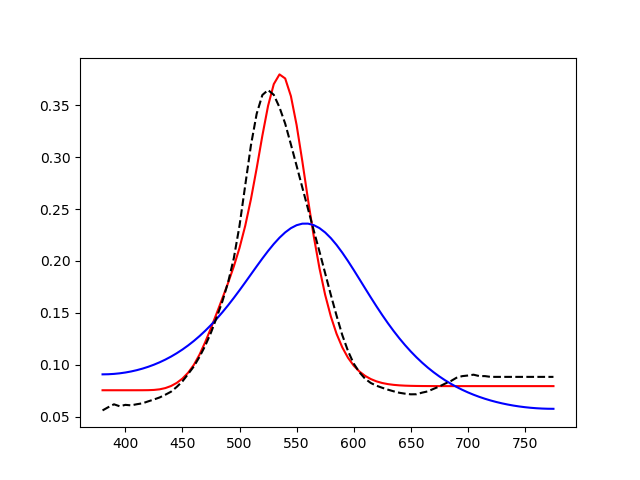
\includegraphics[width=\linewidth]{img/results_techniqueGreen.png}
		\caption{``green'' patch}
		\label{fig:resultsTechnique_green}
	\end{subfigure} \hspace{0.1em}
	\vspace{0.5em}\\
	\begin{subfigure}[t]{0.45\textwidth}
		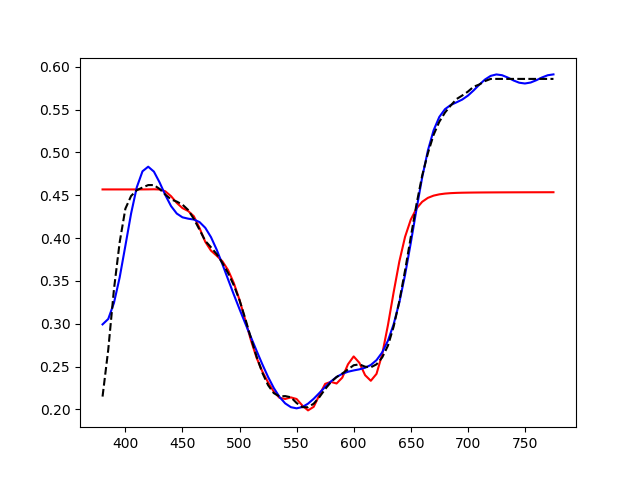
\includegraphics[width=\linewidth]{img/results_techniqueBlueFlower.png}
		\caption{``blue flower'' patch}
		\label{fig:resultsTechnique_blueFlower}
	\end{subfigure} \hspace{0.1em}
	\begin{subfigure}[t]{0.45\textwidth}
		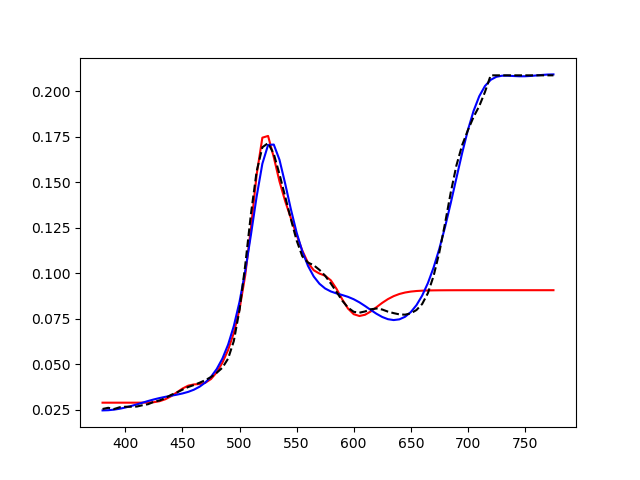
\includegraphics[width=\linewidth]{img/results_techniqueFoliage.png}
		\caption{``foliage'' patch}
		\label{fig:resultsTechnique_foliage}
	\end{subfigure}
	\caption{Comparison between the warped and non-warped reconstructed signal shown on multiple patches of the Macbeth Color Chart}
	\label{fig:resultsTechniques}
\end{figure}

In~\cref{fig:resultsTechniques}, we compare the techniques on a few patches of the Macbeth Color Chart by performing round-trips with 9 coefficients. The difference between the two methods is as mentioned in~\citet{trigonometricMomentsPaper} --- since warping focuses on the more important regions of the spectrum in terms of color perception (i.e. around 550nm), it reconstructs the slight waves in this area quite precisely while neglecting the edges. Non-warping, on the other hand, focuses on the spectra as a whole, which results in approximating the shape over the whole wavelength range but not in an exact replication of any specific spikes.

We cannot definitely determine the more precise method (e.g. warping gives the impression of better performance in case of the ``neutral 5'' patch in~\cref{fig:resultsTechnique_neutral5}, but seems to rather unsuccessful in the case of the ``blue flower'' patch in~\cref{fig:resultsTechnique_blueFlower}). However, the last row of~\cref{table:comparisonMomentTechnique} suggest that although warping performs better on average, its maximum achieved error is higher than that of the non-warping technique.

\begin{figure}[t]
	\centering
	\vspace{1em}
	\begin{subfigure}[t]{0.49\textwidth}
		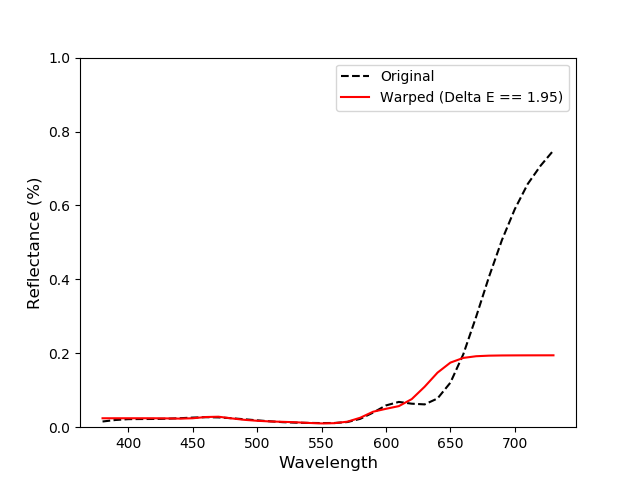
\includegraphics[width=\linewidth]{img/results_worstWarped.png}
		\caption{Warped spectral reconstruction of the Munsell 2.5R 2/6 sample from the Munsell Book of Color, Delta E == 1.95}
		\label{fig:resultWorstWarp}
	\end{subfigure} \hspace{0.1em}
	\begin{subfigure}[t]{0.49\textwidth}
		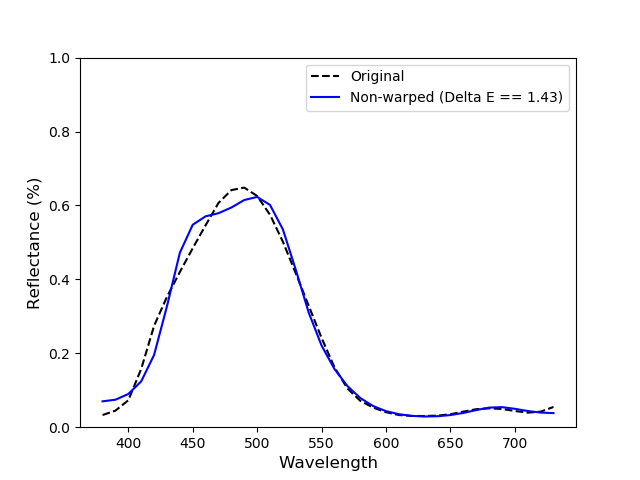
\includegraphics[width=\linewidth]{img/results_worstNonWarped.png}
		\caption{Non-warped spectral reconstruction of the Pantone 3551 C sample of the Pantone color atlas, Delta E == 1.43}
		\label{fig:resultWorstNonWarp}
	\end{subfigure}
	\caption{The worst-case round-trip scenarios of the warped and non-warped technique, 9 coefficients used for spectral reconstruction}
	\label{fig:resultsTechniquesWorst}
\end{figure}

The impact of the worst-case scenario on rendering is another important factor to consider in our decision-making process. Having even one incorrect color could cause significant metameric artifacts, which we want to avoid at all costs. Therefore, we specifically analyze the cases in which the maximum error was obtained. For warping, this represents the Munsell 2.5R 2/6 sample of the Munsell Book of Color, while non-warping performs worst for the Pantone 3551 C sample of the Pantone color atlas. We show the round-trip results of both of these cases in~\cref{fig:resultsTechniquesWorst}.

Although the shortcomings of warping can already be perceived in e.g.~\cref{fig:resultsTechnique_foliage} or~\cref{fig:resultsTechnique_blueFlower}, the failure in the reconstruction of the curve's edges does not have a significant effect of the the resulting RGB color, as the source of color is mainly focused around the middle of the curve. However, if the edges are extremely distinct from the rest of the curve (see~\cref{fig:resultWorstWarp}), they tend to provide unanticipated color information. In such cases, warping the signal presents a disadvantage.

Obviously, the Delta E error caused by unnecessary warping can be reduced to almost 0 by passing the computed coefficients to the optimizer, which then alters the curve so that it evaluates to the correct RGB. However, because we lose the notion of the curve's desired shape and because warping does not focus on the edges, the optimizer is apt to amplify the already existing slight bumps in the middle. This behavior may therefore cause the resulting shape to be extremely distinct from the desired one. 

The non-warping technique, shown in~\cref{fig:resultWorstNonWarp}, is not susceptible to this kind of behavior. Although it creates a rather significant Delta E error, we can observe that the shape of the reconstructed spectrum roughly resembles the original shape. Such a behavior is desired in our case, as the reconstructed reflectance is less prone to cause metameric artifacts under different illuminants. Additionally, as the non-warping technique forces the optimizer to not prioritize specific parts of the curve, the optimization is prone to slightly altering the shape as a whole rather than creating 
irregularities in the middle. Therefore, regardless of the average error, we assume the non-warping technique to outperform warping both when performing simple round-trips, but also if we use this method during the optimization process of fitting the cube.

We put our theory to test. We create a few cubes with varying parameters and we try to fit their entries with both techniques, using the cost functions determined in~\cref{ssec:costFunctions}. We present some of the results in~\cref{fig:resultsTechnique_optimizer}, but we examine many more spectra just to confirm our hypothesis. 

We conclude that our theory is correct --- warping indeed amplifies the slight differences around the middle of the curve in order to achieve the correct color, so much that it creates spikier spectra the more the cube grows. Although this does not necessarily render the cubes created with warped signal useless, it is apparent they are prone to creating memateric artifacts such as the ones presented in~\cref{fig:metamerism}. Additionally, as we already mentioned in ref, the interpolation phase of the rendering pipeline benefits from smooth, non-spiky spectra, which is a criterion the warped spectra do not satisfy. Therefore, we it is save to discard the option of warping.

\begin{figure}[t]
	\centering
	\captionsetup[subfigure]{font=footnotesize,labelfont=footnotesize}
	\captionsetup[subfigure]{justification=centering}
	\begin{subfigure}[t]{0.38\textwidth}
		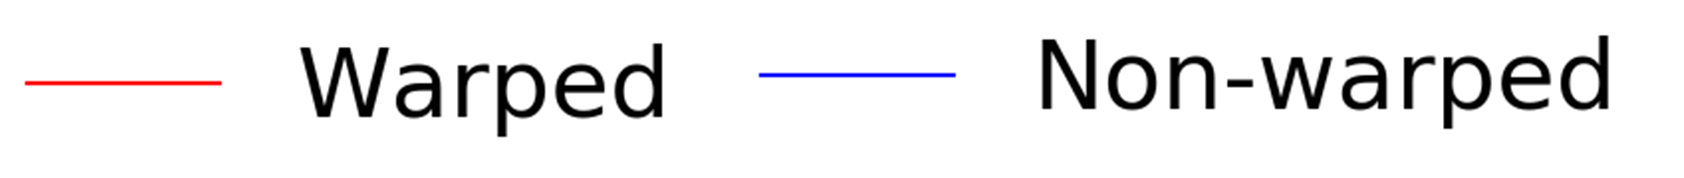
\includegraphics[width=\linewidth]{img/resultsTechniqueOpt_legend.png}
	\end{subfigure} \\
	\begin{subfigure}[t]{0.31\textwidth}
		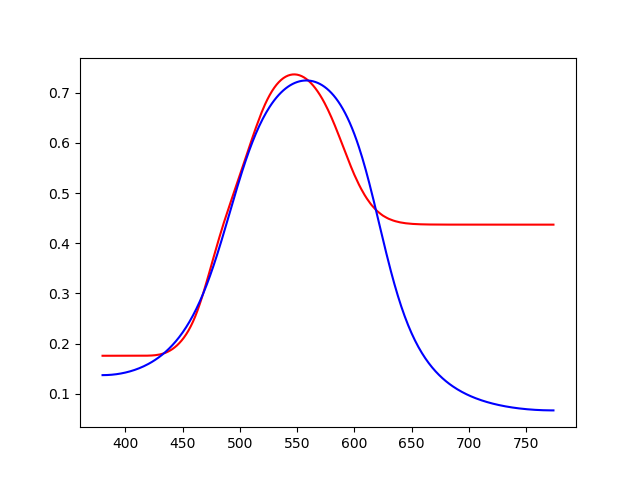
\includegraphics[width=\linewidth]{img/resultsTechniqueOpt_m3_cd64.png}
		\caption{$c=3, cd=64$,\\$RGB=(222.6, 230.7, 230.7)$,\\initial atlas = Macbeth Color Chart}
		\label{fig:resultsTechniqueOpt_m3_cd64}
	\end{subfigure}
	\begin{subfigure}[t]{0.31\textwidth}
		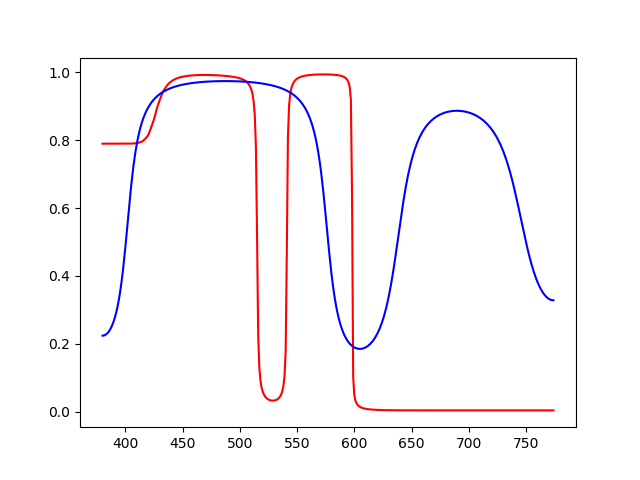
\includegraphics[width=\linewidth]{img/resultsTechniqueOpt_m5_cd32.png}
		\caption{$c=5, cd=32$,\\$RGB=(82.26, 172.74, 255)$,\\initial atlas = Page 14 from Munsell Book of Color}
		\label{fig:resultsTechniqueOpt_m5_cd32}
	\end{subfigure}
	\begin{subfigure}[t]{0.31\textwidth}
		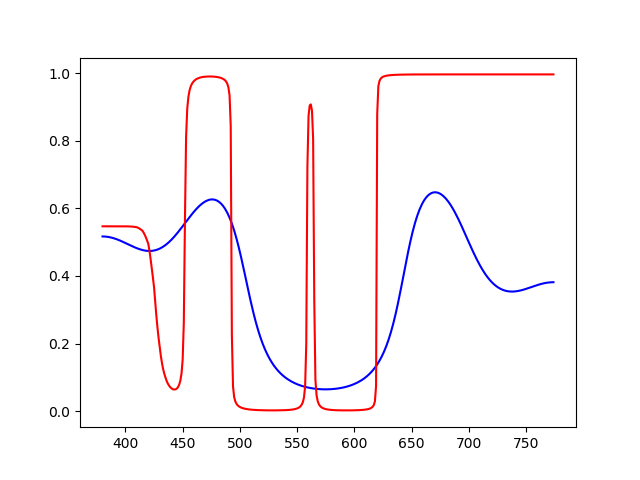
\includegraphics[width=\linewidth]{img/resultsTechniqueOpt_m7_cd16.png}
		\caption{$c=7, cd=16$,\\$RGB=(102, 17, 153)$,\\ fitted from middle}
		\label{fig:resultsTechniqueOpt_m7_cd16}
	\end{subfigure} 
	\caption{Comparison of warping and non-warping when used for fitting cubes, shown on cube entries from different cubes}
	\label{fig:resultsTechnique_optimizer}
\end{figure}

Obviously, the ideal solution would be to store the spectra with the method that provides better Delta E error and use non-warping for cube fitting afterwards. However, such an approach is impractical. Firstly, currently, as the first step of the spectral reconstruction is the conversion of wavelength array to a phase signal, using only one method means we can save this signal prior to fitting and reuse it, thus lowering time complexity. Using both methods would require either storing two phase signals, or recomputing them during each reconstruction. Secondly, as we use non-warping for cube fitting anyway, saving only some atlas entries with warping would be both impractical and would not provide too many benefits. Therefore, we leave the possibility of implementation of the support of both methods as future work.

\subsection{Cost functions} \label{ssec:costFunctions}

In addition to the moment storage technique, another thing greatly affecting the performance of the fitting are the cost functions of optimizer. For the fitting of the sigmoids, Borgtool uses three cost functions, or \emph{residuals}, each of them specifying the absolute color difference in one axis of the RGB cube. Such an approach has outperformed both the Euclidean color distance and even the Delta E difference --- the higher the number of meaningful residuals, the more information about the coefficients' behavior can the optimizer deduce, which, in turn, results in faster and more precise convergence to global optimum.

We therefore copy this approach to specify the color difference. In case of fitting of the regular lattice points (performed in step ref cube fitting), the obtained results are satisfactory. However, a problem occurs upon fitting the atlas lattice points (see step2).

As already mentioned in ref, the process of seeding the cube with an atlas assigns each atlas entry its closest lattice point (atlas lattice point) in the cube. The distance between the atlas entry and its atlas lattice point is dependent on the size of the voxel. Although it can be zero, the chances of that happening for every point of the atlas are slim. This implies that the points' curves cannot be exactly the same --- on the contrary, slight differences between them are even necessary.

The current cost functions, however, take into account the RGB differences only. They do not try to reconstruct similar shapes in any way, which, in turn, may result in significant shape errors in the resulting spectra. This behavior is not as perceivable in higher-dimensional cubes (e.g. 64), where the starting color difference is so low it does not allow the optimizer to change the reconstructed spectrum a lot before it converges. However, lower-dimensional cubes (e.g. 32) are prone to such behavior. Furthermore, as the specified coefficients are in their nature Fourier coefficients, the optimizer is apt to create spectra in the form of multiple waves with a rather high amplitude, which is only amplified the greater the color difference is.

\begin{figure}[t]
	\centering
	\captionsetup[subfigure]{font=footnotesize,labelfont=footnotesize}
	\captionsetup[subfigure]{justification=centering}
	\begin{subfigure}[t]{0.70\textwidth}
		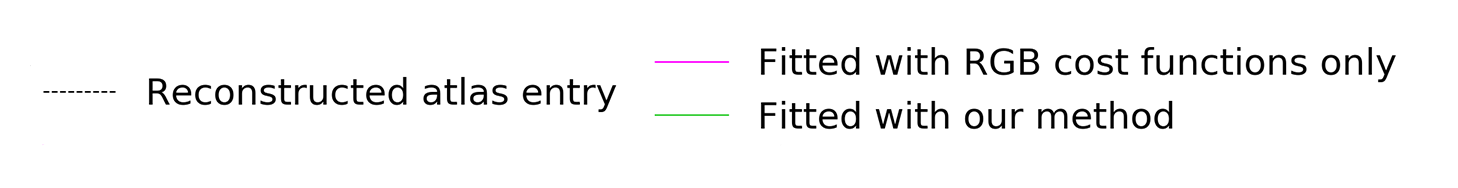
\includegraphics[width=\linewidth]{img/results_costFunctions_legend.png}
	\end{subfigure} \\
	\begin{subfigure}[t]{0.45\textwidth}
		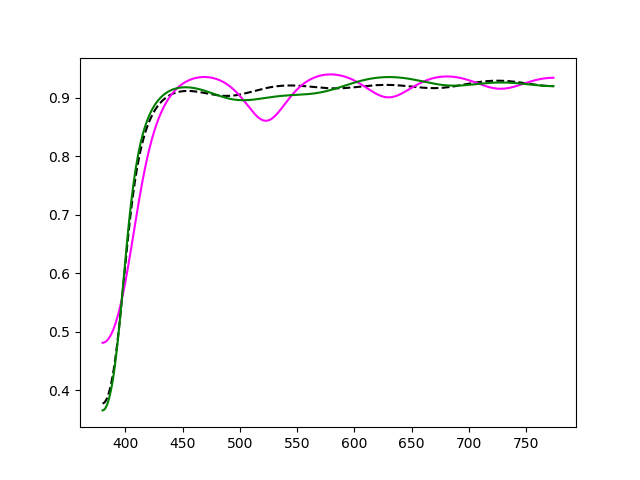
\includegraphics[width=\linewidth]{img/results_costFunctions_white_cd32.png}
		\caption{``white'' patch, CD = 32, $d = 5.81$}
		\label{fig:resultsCostFunctions_white32}
	\end{subfigure} \hspace{0.1em}
	\begin{subfigure}[t]{0.45\textwidth}
		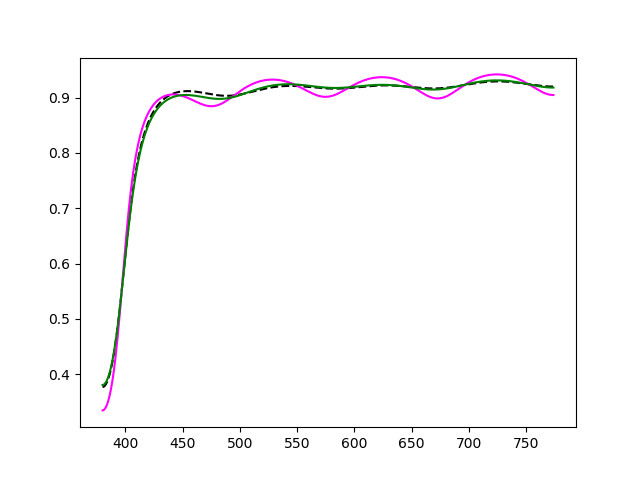
\includegraphics[width=\linewidth]{img/results_costFunctions_white_cd64.png}
		\caption{``white'' patch, CD = 64, $d = 1.99$}
		\label{fig:resultsCostFunctions_white64}
	\end{subfigure} \hspace{0.1em}
	\vspace{0.5em}\\
	\begin{subfigure}[t]{0.45\textwidth}
		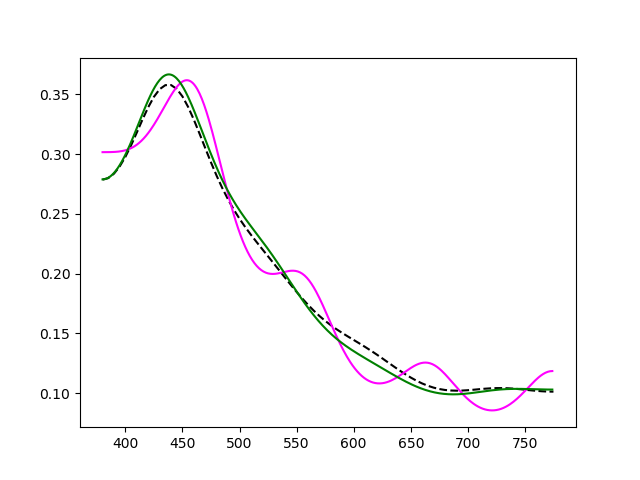
\includegraphics[width=\linewidth]{img/results_costFunctions_bs_cd32.png}
		\caption{``blue sky'' patch, CD = 32, $d = 4.1$}
		\label{fig:resultsCostFunctions_bs32}
	\end{subfigure} \hspace{0.1em}
	\begin{subfigure}[t]{0.45\textwidth}
		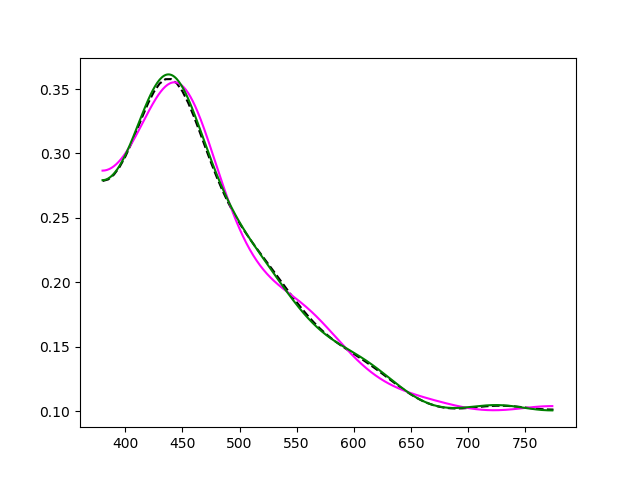
\includegraphics[width=\linewidth]{img/results_costFunctions_bs_cd64.png}
		\caption{``blue sky'' patch, CD = 64, $d = 0.96$}
		\label{fig:resultsCostFunctions_bs64}
	\end{subfigure}
	\caption{Comparison between the RGB cost functions and our method for fitting main atlas lattice points}
	\label{fig:resultsCostFunctions}
\end{figure}

We show an example of such behavior in~\cref{fig:resultsCostFunctions}, where we attempt to fit both the ``white'' and the ``blue sky'' patches of the Macbeth Color Checker to their main atlas lattice points in both a 32 and a 64-dimensional cube. The magenta plot represents the results of fitting with only the three cost functions, which is definitely undesired.

Note that we compare the optimized spectra not with the original atlas spectra, but with the spectra that is reconstructed from the original's coefficients. That way we can keep track of the optimizer's ability to mimic its input.

When fitting other spectral data, the optimizer does not behave as drastically as shown in~\cref{fig:resultsCostFunctions}. On the contrary, many fitted altas entries (such as the ``blue flower'' of the Macbeth Color Checker) resemble their input quite well. However, we must focus on the worst-case scenario as we do not wish to experience any metameric artifacts, not even in one color.

There are two ways of solving the presented problem --- either by simply using a higher-dimensional cube, or by adding cost functions that force the optimizer to keep the difference between the original and the reconstructed curve as low as possible.

We incline towards using more cost functions, both because the use of a higher-dimensional cube would require greater processing time, but also because the optimizer is prone to creating wave-like spectra nonetheless, even if the waves have much lower amplitude.

Our first idea was to add a fourth residual that would specify the least square error between the curves. Although the results with this method were quite satisfactory, the optimizer was sometimes prone to spikes, as the error was computed over the spectra as a whole rather. We therefore added one residual for each pair of spectral samples, which, in our case (as we sample with an increment of 1) sums up to roughly 400 cost functions. This allows the optimizer to specifically focus on the samples that it wants lowered, which therefore eliminates the possibility of spikes.

Although having this many residuals may seem far-fetched, the optimizer handles it well. It also does not reduce the importance of the three color cost functions. Its only notable issue is that it is prone to declaring optimization failures even if the residuals are satisfactory. This is due to its need to minimize all the residuals so they approach zero. However, we know that the original and resulting reflectance curves can not be exactly the same.

We solve this problem by adding a simple threshold to the optimizer. In case the least square error between one spectral sample pair is lower, the optimizer assumes it to be zero and is not concerned by it anymore. Initially, we set the threshold to zero, but increase it if the optimizer fails and try again. 

The heuristic regarding the threshold does not, on average, need to be invoked more than 2-3 times when fitting an arbitrary atlas to a sufficiently-sized cube (i.e. 64-dimensional). It is clear that by lowering the cube's dimension, the heuristic becomes more utilized. For example, for an 8-dimensional cube, it reaches up to 100 invocations, and even then the fitting may not always be successful.

We, however, do not concern ourselves much with cubes of such low dimension --- even for a 32-dimensional cube, the difference between an atlas lattice point and an atlas entry can be as much as $d = 13.86$ (in which $d$ denotes the Euclidean distance), which already suggests a rather significant difference between reflectance spectra and therefore implies loss of atlas information. We therefore strongly recommend the user to avoid cubes of low dimensions (i.e. under 32).

In~\cref{fig:resultsCostFunctions}, we provide a comparison between the results obtained with our cost functions and the results obtained with the original ones. It is clear that our approach is superior in terms of spectral shape and, as the implementation of the color specifying residuals is identical in both approaches, the resulting RGB values are extremely similar. We therefore use our newly presented residuals for atlas fitting.

Our cost functions give us the ability to control the shape of the resulting spectra. By further utilizing them, we could fit the neighbors of atlas lattice points so that their spectra is extremely similar. Applying this method to the whole cube-fitting process could therefore create an uplifting model with a rather uniform spectra. Such an uplifting model is especially desired for the interpolation phase in rendering.

However, two problems already arise with this approach. Firstly, by growing the cube from multiple atlas entries at the same time, there is bound to be a point in which neighbors are fitted from different prior atlas entries. By our premise, this would mean that the spectra of these two points could be vastly different.

Another issue is the significant increase in time complexity. Even excluding the complex calculations the optimizer must perform during minimization, the computation of around 400 residuals takes a lot more time than just computing the original 3. The process of fitting a 32-dimensional cube, regardless of the number of its moments and the allowed optimizer's threshold, then takes hours instead of mere minutes when executed on an ordinary desktop PC. This renders our cost functions unusable for cube fitting and we must therefore settle for using the RGB cost functions only.

The increased time complexity gives rise to the question of whether it is even feasible to use our cost functions for atlas fitting. It is true that in some cases, for example when seeding with the Munsell Color Atlas, in which the atlas lattice points make up a significant portion of the cube, the time difference is noticeable. However, if we wish to seed the cube with all the atlas entries, we often require a cube of a much higher dimension, the fitting of which diminishes the time importance of the initial atlas fit. Although this may not be true in all cases (e.g. we could create an atlas the size of the cube with each entry mapping to a different lattice point), it is still beneficial to trade off the possibility of a higher time complexity for much precise spectra.

Therefore, we use the original RGB difference cost functions for fitting regular point and our new cost functions for fitting atlas lattice point.

\subsection{Number of moments}
 
Maybe add a section about unfittable cubes?

However, correct round-trips are not the only factor we need to take into consideration when fitting the cube. We also need to focus on both the \emph{smoothness of the resulting spectra} and the \emph{behavior of the optimizer} under the current technique.

The smoothness of the spectra is especially important for the interpolation process that takes place during the rendering. Interpolating multiple spiky, non-similar spectra would result in similarly uneven spectra, which, in addition to incorrect color, may be susceptible to extreme metameric artifacts.  

The behavior of the optimizer also plays a big role. During the optimization, it takes into account only the resulting RGB of the curve rather than the shape of the curve itself. Therefore, it does not aim for a curve with a similar shape than its neighbor, which may likewise cause issues during the interpolation.

When we fit from the middle, we only aim for the smoothness of the resulting spectra and for the behavior of the optimizer. We therefore want as less coefficients as possible and, as we do not care about round trips, we can use any of the techniques available.

We already said that using 9 coefficients is unecessary, as 3 already create rather smooth spectra that is way better for interpolation. However, we here find out that it is not only unnecessary but extremely discouraged. We can see in the image how the fitting proceeds. It amplifies the already existing wave-like patterns, exhibiting the same behavior as it did during atlas fitting, which is caused by the cost functions not considering the shape of the resulting spectra. By allowing only three coefficients, we limit the optimizer so it must create smooth spectra and it cannot create crazy shapes. Additionaly, it is better for performance - fiting of a 9-coefficients takes around blabla, while fitting 3 takes blabla. We provide measurements here? of performance

Although we cannot control shape, we can control smoothness. We want smooth spectra both for interpolation purposes and because smooth spectra is less prone to metameric artifacts, see chapter 1.

The behavior we talked about before of the optimizer is a problem 
It would be extremely beneficial for the

For middle fitting, we always recommend 2 moments, 3 coeffs due to the runtime. Moreover, they are very smooth but not straight which is ideal for our purposes. Obviously, we can fit with higher but that takes a lot of time and does not provide any advantage. The default setting is therefore 3 coefs, 2 moments.

Obviously, fitting with these causes metameric artifacts, similar to the ones created by sigmoid, we show these in PICTURE. We can also show metameric artifacts when fitting with more? (try this maybe)

Another slight trick is to use a lower number of coefficients - we therefore do not get as big artifacts because we cannot possibly reconstruct such crazy spectra with low number of coefficients. 

The optimizer is always faster for lower number of coefficients as it does not need to change them up as much. Also faster but does not change them so much SO it results in spectrum that is similar to the first one. However, we cannot possibly simulate the curve with only the limited number of coefficients, the table says so. Therefore we must find something in the middle. We try not to focus on performance here because obviously, fitting anything that is higher than 32 takes hours and we want to have it look the best way we can.

\section{Performace}

heuristics performance, overall runtime of the cube

\section{Rendering}

- which technique gives the best results (metamerism results)


Also mention that it is multi-threaded and performance is not really a priority - the cube has to be created only once and then can be reused as much as the artists need.


\chapter*{Conclusion}
\addcontentsline{toc}{chapter}{Conclusion}


However, it has to be noted that the approach presented in this paper works perfectly fine for target spectra sets up to several dozen, or maybe even low numbers of hundred, data points. Which is sufficient for typical usage in VFX scenarios, where only a few key assets (like e.g. the main colours of the costume of a lead character) are measured on set, in order to later constrain the spectral uplift of virtual doubles of this character.
We also note that our approach, while being both slower to fit and slower to render than the sigmoid technique, offers the unique capability of targeted uplifting, which was simply not available before. As such, we deem a somewhat slower performance compared to sigmoid-based uplift to be an acceptable price to pay.

%%% Bibliography
%%% Bibliography (literature used as a source)
%%%
%%% We employ bibTeX to construct the bibliography. It processes
%%% citations in the text (e.g., the \cite{...} macro) and looks up
%%% relevant entries in the bibliography.bib file.
%%%
%%% The \bibliographystyle command selects, which style will be used
%%% for references from the text. The argument in curly brackets is
%%% the name of the corresponding style file (*.bst). Both styles
%%% mentioned in this template are included in LaTeX distributions.

\bibliographystyle{plainnat}    %% Author (year)
% \bibliographystyle{unsrt}     %% [number]

\renewcommand{\bibname}{Bibliography}

%%% Generate the bibliography. Beware that if you cited no works,
%%% the empty list will be omitted completely.

\bibliography{bibliography}

%%% If case you prefer to write the bibliography manually (without bibTeX),
%%% you can use the following. Please follow the ISO 690 standard and
%%% citation conventions of your field of research.

% \begin{thebibliography}{99}
%
% \bibitem{lamport94}
%   {\sc Lamport,} Leslie.
%   \emph{\LaTeX: A Document Preparation System}.
%   2nd edition.
%   Massachusetts: Addison Wesley, 1994.
%   ISBN 0-201-52983-1.
%
% \end{thebibliography}


%%% Figures used in the thesis (consider if this is needed)
%%\listoffigures

%%% Tables used in the thesis (consider if this is needed)
%%% In mathematical theses, it could be better to move the list of tables to the beginning of the thesis.
%%\listoftables

%%% Abbreviations used in the thesis, if any, including their explanation
%%% In mathematical theses, it could be better to move the list of abbreviations to the beginning of the thesis.
%%\chapwithtoc{List of Abbreviations}

%%% Attachments to the master thesis, if any. Each attachment must be
%%% referred to at least once from the text of the thesis. Attachments
%%% are numbered.
%%%
%%% The printed version should preferably contain attachments, which can be
%%% read (additional tables and charts, supplementary text, examples of
%%% program output, etc.). The electronic version is more suited for attachments
%%% which will likely be used in an electronic form rather than read (program
%%% source code, data files, interactive charts, etc.). Electronic attachments
%%% should be uploaded to SIS and optionally also included in the thesis on a~CD/DVD.
%%% Allowed file formats are specified in provision of the rector no. 72/2017.
\appendix
\chapter{Software user guide}
\chapter{Attachments}

\section{Delta E error caused by moment sampling} \label{sec:completeMomentError}

\begin{table}[h]
	\centering
	\begin{tabular}{crrrrrrrr}
		\toprule
		\multirow{4}{*}{Moments} &
		\multicolumn{8}{c}{Methods} \\
		\cmidrule(lr){2-9}
		&\multicolumn{2}{c}{M\&W} &
		\multicolumn{2}{c}{M\&nonW} &
		\multicolumn{2}{c}{nMW} &
		\multicolumn{2}{c}{nMnW}\\
		\cmidrule(lr){2-9}
		& Avg & Max & Avg & Max & Avg & Max & Avg & Max \\
		\cmidrule(lr){1-9}
		0&23.88&130.27&23.95&130.62&23.86&130.38&23.95&130.62\\
		1&13.09&97.76&16.92&107.23&4.08&51.23&8.48&67.12\\
		2&1.39&21.71&10.18&74.62&1.31&20.87&2.56&20.14\\
		3&0.74&7.43&6.3&60.36&0.71&8.18&0.89&6.36\\
		4&0.49&5.46&2.58&26.36&0.61&5.16&0.46&3.62\\
		5&0.35&3.95&1.1&6.83&0.47&4.11&0.37&3.2\\
		6&0.31&3.19&0.73&6.12&0.32&3.07&0.27&2.73\\
		7&0.28&2.85&0.71&5.67&0.29&2.28&0.24&2.26\\
		8&0.27&2.42&0.61&3.94&0.29&1.89&0.23&1.52\\
		9&0.21&2.41&0.43&3.78&0.27&1.8&0.19&1.1\\
		10&0.21&2.41&0.26&2.62&0.28&1.81&0.18&1.28\\
		11&0.17&2.4&0.2&2.26&0.29&1.81&0.16&1.07\\
		12&0.17&2.39&0.2&2.32&0.27&1.64&0.15&1.09\\
		13&0.16&2.36&0.2&2.29&0.25&1.58&0.15&1.09\\
		14&0.16&2.32&0.2&1.93&0.24&1.56&0.16&1.09\\
		15&0.15&2.26&0.18&1.2&0.2&2.66&0.16&1.09\\
		16&0.15&2.23&0.17&1.17&0.21&4.3&0.15&1.08\\
		17&0.15&2.21&0.15&1.12&0.25&4.27&0.14&1.08\\
		18&0.15&2.19&0.14&1.12&0.29&3.3&0.14&1.08\\
		19&0.15&2.16&0.14&1.08&0.44&4.04&0.14&1.08\\
		20&0.15&2.12&0.14&1.07&0.57&4.24&0.15&1.07\\
		21&0.15&2.06&0.14&1.08&0.65&3.42&0.15&1.08\\
		22&0.15&2.01&0.14&1.08&0.37&2.53&0.14&1.09\\
		23&0.15&1.98&0.14&1.09&0.36&2.16&0.14&1.1\\
		24&0.15&1.96&0.14&1.09&0.22&1.44&0.14&1.12\\
		25&0.16&1.95&0.14&1.09&0.22&1.17&0.15&1.14\\
		26&0.16&1.93&0.14&1.09&0.19&1.04&0.16&1.19\\
		27&0.16&1.9&0.14&1.09&0.24&1.11&0.16&1.24\\
		28&0.16&1.87&0.14&1.09&0.19&0.84&0.15&1.29\\
		29&0.17&1.82&0.14&1.09&0.14&0.97&0.13&0.94\\
		30&0.17&1.78&0.13&1.09&0.15&0.99&0.16&1.13\\
		31&0.18&1.94&0.14&1.09&0.16&1.04&0.21&1.59\\
		32&0.19&1.89&0.14&1.09&0.15&0.9&0.29&1.62\\
		33&0.21&1.76&0.14&1.09&0.13&0.95&0.27&1.62\\
		34&0.21&1.86&0.14&1.09&0.13&1.26&0.2&1.46\\
	35&0.19&1.79&0.14&1.09&0.16&1.84&0.23&1.17\\
	36&0.2&1.82&0.14&1.09&0.16&1.71&0.22&1.19\\
	37&0.16&1.79&0.14&1.09&0.19&1.82&0.15&1.08\\
	38&0.11&1.77&0.14&1.09&0.23&2.23&0.1&0.72\\
	39&0.12&1.67&0.14&1.09&0.34&2.28&0.07&0.73\\
	40&0.13&1.68&0.14&1.09&0.27&1.54&0.06&0.73\\
		\bottomrule
	\end{tabular}
	\label{table:completeMomentError}
\end{table}

\openright
\end{document}
